\documentclass[text.tex]{subfiles}

\begin{document}
\section{Two dimensional quasicrystal}
Now that we have analyzed quasicrystals with one dimensional windows and perhaps more importantly we have seen our method of analysis in action it is time to analyze quasicrystals with two dimensional windows. 

First we recapitulate various components of our quasicrystal model (in its entirety in Definition \ref{def_quasicrystal}). 

Let $n\in\NN\setminus\{2,3,4,6\}$. Let $\beta$ be a quadratic Pisot-cyclotomic number of order $n$, associated to $\rho = 2\cos\left(2\pi/n\right)$. Further, let $\ast:\RR^2\to\RR^2$ be defined as $(x,y)^\ast = (\Re{\big((x+iy)^{\ast^\CC}\big)}, \Im{\big((x+iy)^{\ast^\CC}\big)})$ where $\ast^\CC$ is an appropriate Galois isomorphism of $\zeta = e^{2\pi \i/n}$. 
Let $v_1, v_2\in\RR^2$:
$$v_1=(1,0)\quad\text{and}\quad v_2 = (\Re{(\zeta)}, \Im{(\zeta)})$$
and let $M = \ring v_1+\ring v_2$ and $N = \ring v_1^\ast+\ring v_2^\ast$.
Lastly let $\Omega\subset N$ be bounded with nonempty interior. 

The model of two dimensional quasicrystal linked to irrationality $\beta$ and window $\Omega$ is the set:
$$\quasi{\Omega} = \{ x \in M\; |\; x^\ast\in \Omega\}$$

We will use the notation from above to denote the same objects in the rest of this chapter. 

\begin{figure}[h!]
\centering
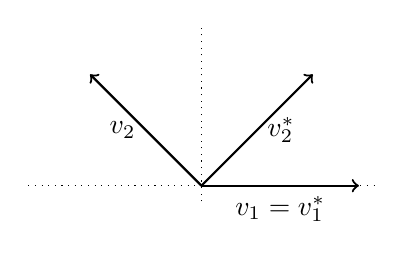
\begin{tikzpicture}[scale=2]
\draw [dotted] (0,-0.1) -- (0,1);
\draw [dotted] (-1.1,0) -- (1.1,0);

\draw [thick,->] (0,0) -- node[below] {$v_1 = v_1^\ast$} (1,0);
\draw [thick,->] (0,0) -- node[left] {$v_2$} (-0.707106781,0.707106781);
\draw [thick,->] (0,0) -- node[right] {$v_2^\ast$} (0.707106781,0.707106781);
\end{tikzpicture}
\caption{Example of the vectors $v_1$, $v_2$, $v_1^\ast$ and $v_2^\ast$ for Pisot-cyclotomic $\beta_8=1+\sqrt{2}$.}
\end{figure}

As we hinted before we will analyze two dimensional quasicrystals just for several specific windows. 
\begin{definition}
Let $\Omega\subset\RR^2$:\\
$\Omega = Iv_1^\ast+Iv_2^\ast$ where $I$ is a left-closed right-open interval is a \textbf{rhombic window}. \\
$\Omega$ equal to closed convex hull of $\big\{\big(\cos(2k\pi/n),\sin(2k\pi/n)\big)\big| k = 0,\dots,n-1 \big\}$ for $n\in\NN$ is a \textbf{$n$-gonal window}. \\ 
$\Omega = \{x\in\RR^2\,|\,\lVert x \rVert \leq R\}$ where $R>0$ is a \textbf{circular window}.
\end{definition}

\begin{figure}[h!]
\centering
\begin{tikzpicture}[scale=2]
\draw [opacity=0.5] (0.823553391, 0.353553390) -- (0.883553391, 0.353553390);
\draw [opacity=0.5] (0.853553391, 0.323553390) -- (0.853553391, 0.383553390);
\draw (0,0) --  (1,0) -- (1.707106781,0.707106781) -- (0.707106781,0.707106781) -- cycle;
\draw [opacity=0] ($(0,0.47443)+(0.853553391, 0.353553390)$) -- ($(0,-0.47443)+(0.853553391, 0.353553390)$);
\end{tikzpicture}
\begin{tikzpicture}[scale=2]
\draw [opacity=0.5] (-0.03, 0) -- (0.03, 0);
\draw [opacity=0.5] (0, -0.03) -- (0, 0.03);
\draw (0.47443,0) -- (0.33547,0.33547) -- (0,0.47443) -- (-0.33547,0.33547) --  (-0.47443,0) -- (-0.33547,-0.33547) -- (0,-0.47443) -- (0.33547,-0.33547) -- cycle;
\draw [opacity=0] (-0.85355,0) -- (0.85355,0);
\end{tikzpicture}
\begin{tikzpicture}[scale=2]
\draw [opacity=0.5] (-0.03, 0) -- (0.03, 0);
\draw [opacity=0.5] (0, -0.03) -- (0, 0.03);
\draw (0,0) circle[radius=0.47443];
\draw [opacity=0] (-0.85355,0) -- (0.85355,0);
\end{tikzpicture}
\caption{Example of three window shapes: rhombic, octagonal and circular windows for Pisot-cyclotomic $\beta_8=1+\sqrt{2}$.}
\end{figure}

Now we explain why we did analyze the one dimensional quasicrystal first. Since we used cut-and-project scheme for our model of a quasicrystal it is possible to decompose a quasicrystal with rhombic window into two quasicrystals with one dimensional windows. 
$$\quasi{Iv_1^\ast+Iv_2^\ast} = \quasi{I}v_1+\quasi{I}v_2$$
Here we see why a rhombic window has different closeness to the other windows we consider, it stems right from this decomposition and the left-closed right-open intervals.

Equipped with this very handy decomposition we are ready to start the analysis of two dimensional quasicrystal with the first step. 

\subsection{Arbitrary finite section}
There are two concepts vitally important to this step. The decomposition we just saw and the inclusion property. First let us explain how to acquire arbitrary finite section of a quasicrystal with a rhombic window. 

\begin{enumerate}
\item[Input:] rhombic window $Iv_1^\ast+Iv_2^\ast$; finite intervals $[x_1,x_2]$, $[y_1,y_2]$
\item acquire finite section of one dimensional quasicrystal with window $I$ and interval $[x_1,x_2]$, save in \texttt{quasicrystal01}
\item acquire finite section of one dimensional quasicrystal with window $I$ and interval $[y_1,y_2]$, save in \texttt{quasicrystal02}
\item compose list \texttt{quasicrystal} as points $z=x\cdot v_1+y\cdot v_2$ for $x\in$ \texttt{quasicrystal01} and $y\in$ \texttt{quasicrystal02}
\item[Output:] the list \texttt{quasicrystal}
\end{enumerate}

This algorithm however might not work as we expect. Since $v_1$ and $v_2$ are not perpendicular the returned finite section is not the intersection of the quasicrystal with a rectangle (i.e.\ $\quasi{Iv_1^\ast+Iv_2^\ast}\cap[x_1,x_2]\times[y_1,y_2]$) but is also of the shape of a rhombus. This is simply solved by acquiring larger finite section and cropping it to fit the desired rectangle. There is an example of such finite section in Figure \ref{fig_quasicrystalExampleRhombus}. 

\begin{figure}[h!]
\centering
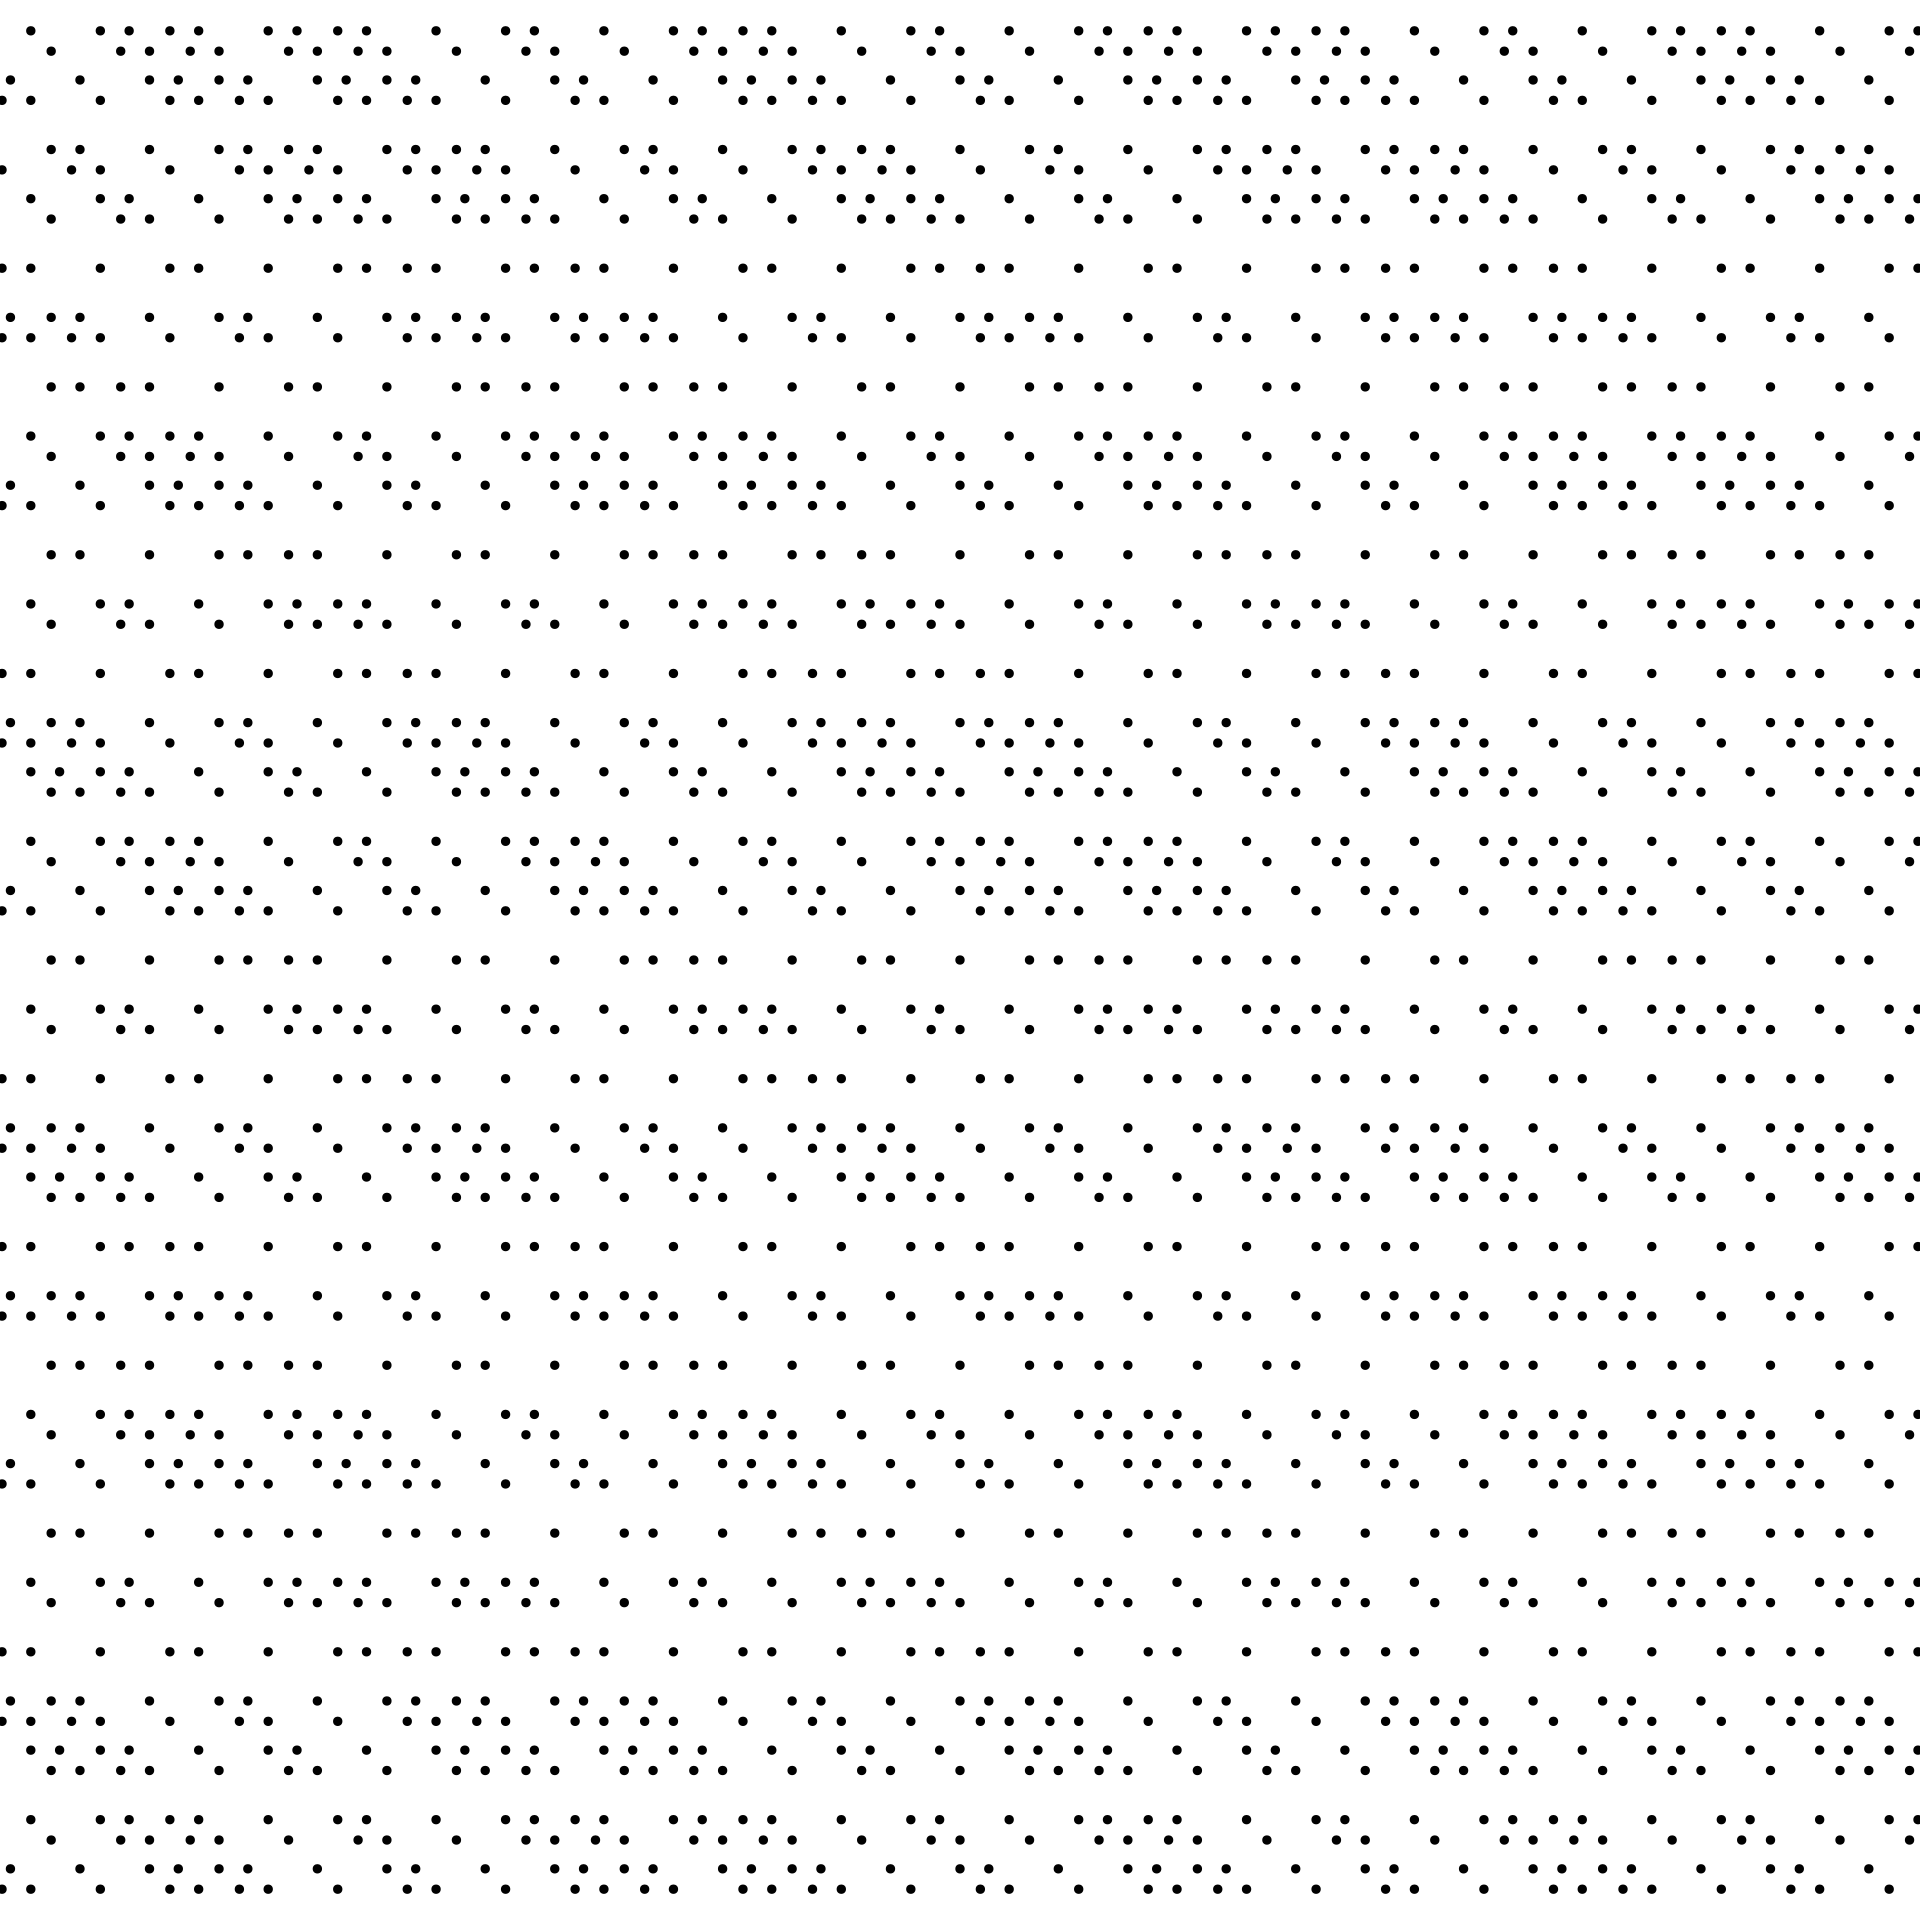
\includegraphics[width=0.9\textwidth]{img/2D/rhombus}
\caption{Example of a finite section of a two dimensional quasicrystal with a rhombic window for Pisot-cyclotomic $\beta_8=1+\sqrt{2}$.}
\label{fig_quasicrystalExampleRhombus}
\end{figure}

Now we use the inclusion property to generalize the algorithm for any window $\Omega$. As a reminder the inclusion property is: 
$$\Omega_1\subset\Omega_2 \quad\Rightarrow\quad \quasi{\Omega_1}\subset\quasi{\Omega_2}$$
Thus it is enough to circumscribe a rhombus $(Iv_1^\ast+Iv_2^\ast)$ to whatever window we desire, use the algorithm to acquire a finite section of a quasicrystal with the rhombic window and then check for each point whether its star map image fits inside the desired window: 
$$\quasi{\Omega} = \{ x \in \quasi{Iv_1^\ast+Iv_2^\ast}\; |\; x^\ast\in \Omega\}$$
There is an example of this process in Figure \ref{fig_quasicrystalExampleOctagon}. 

\begin{figure}[h!]
\centering
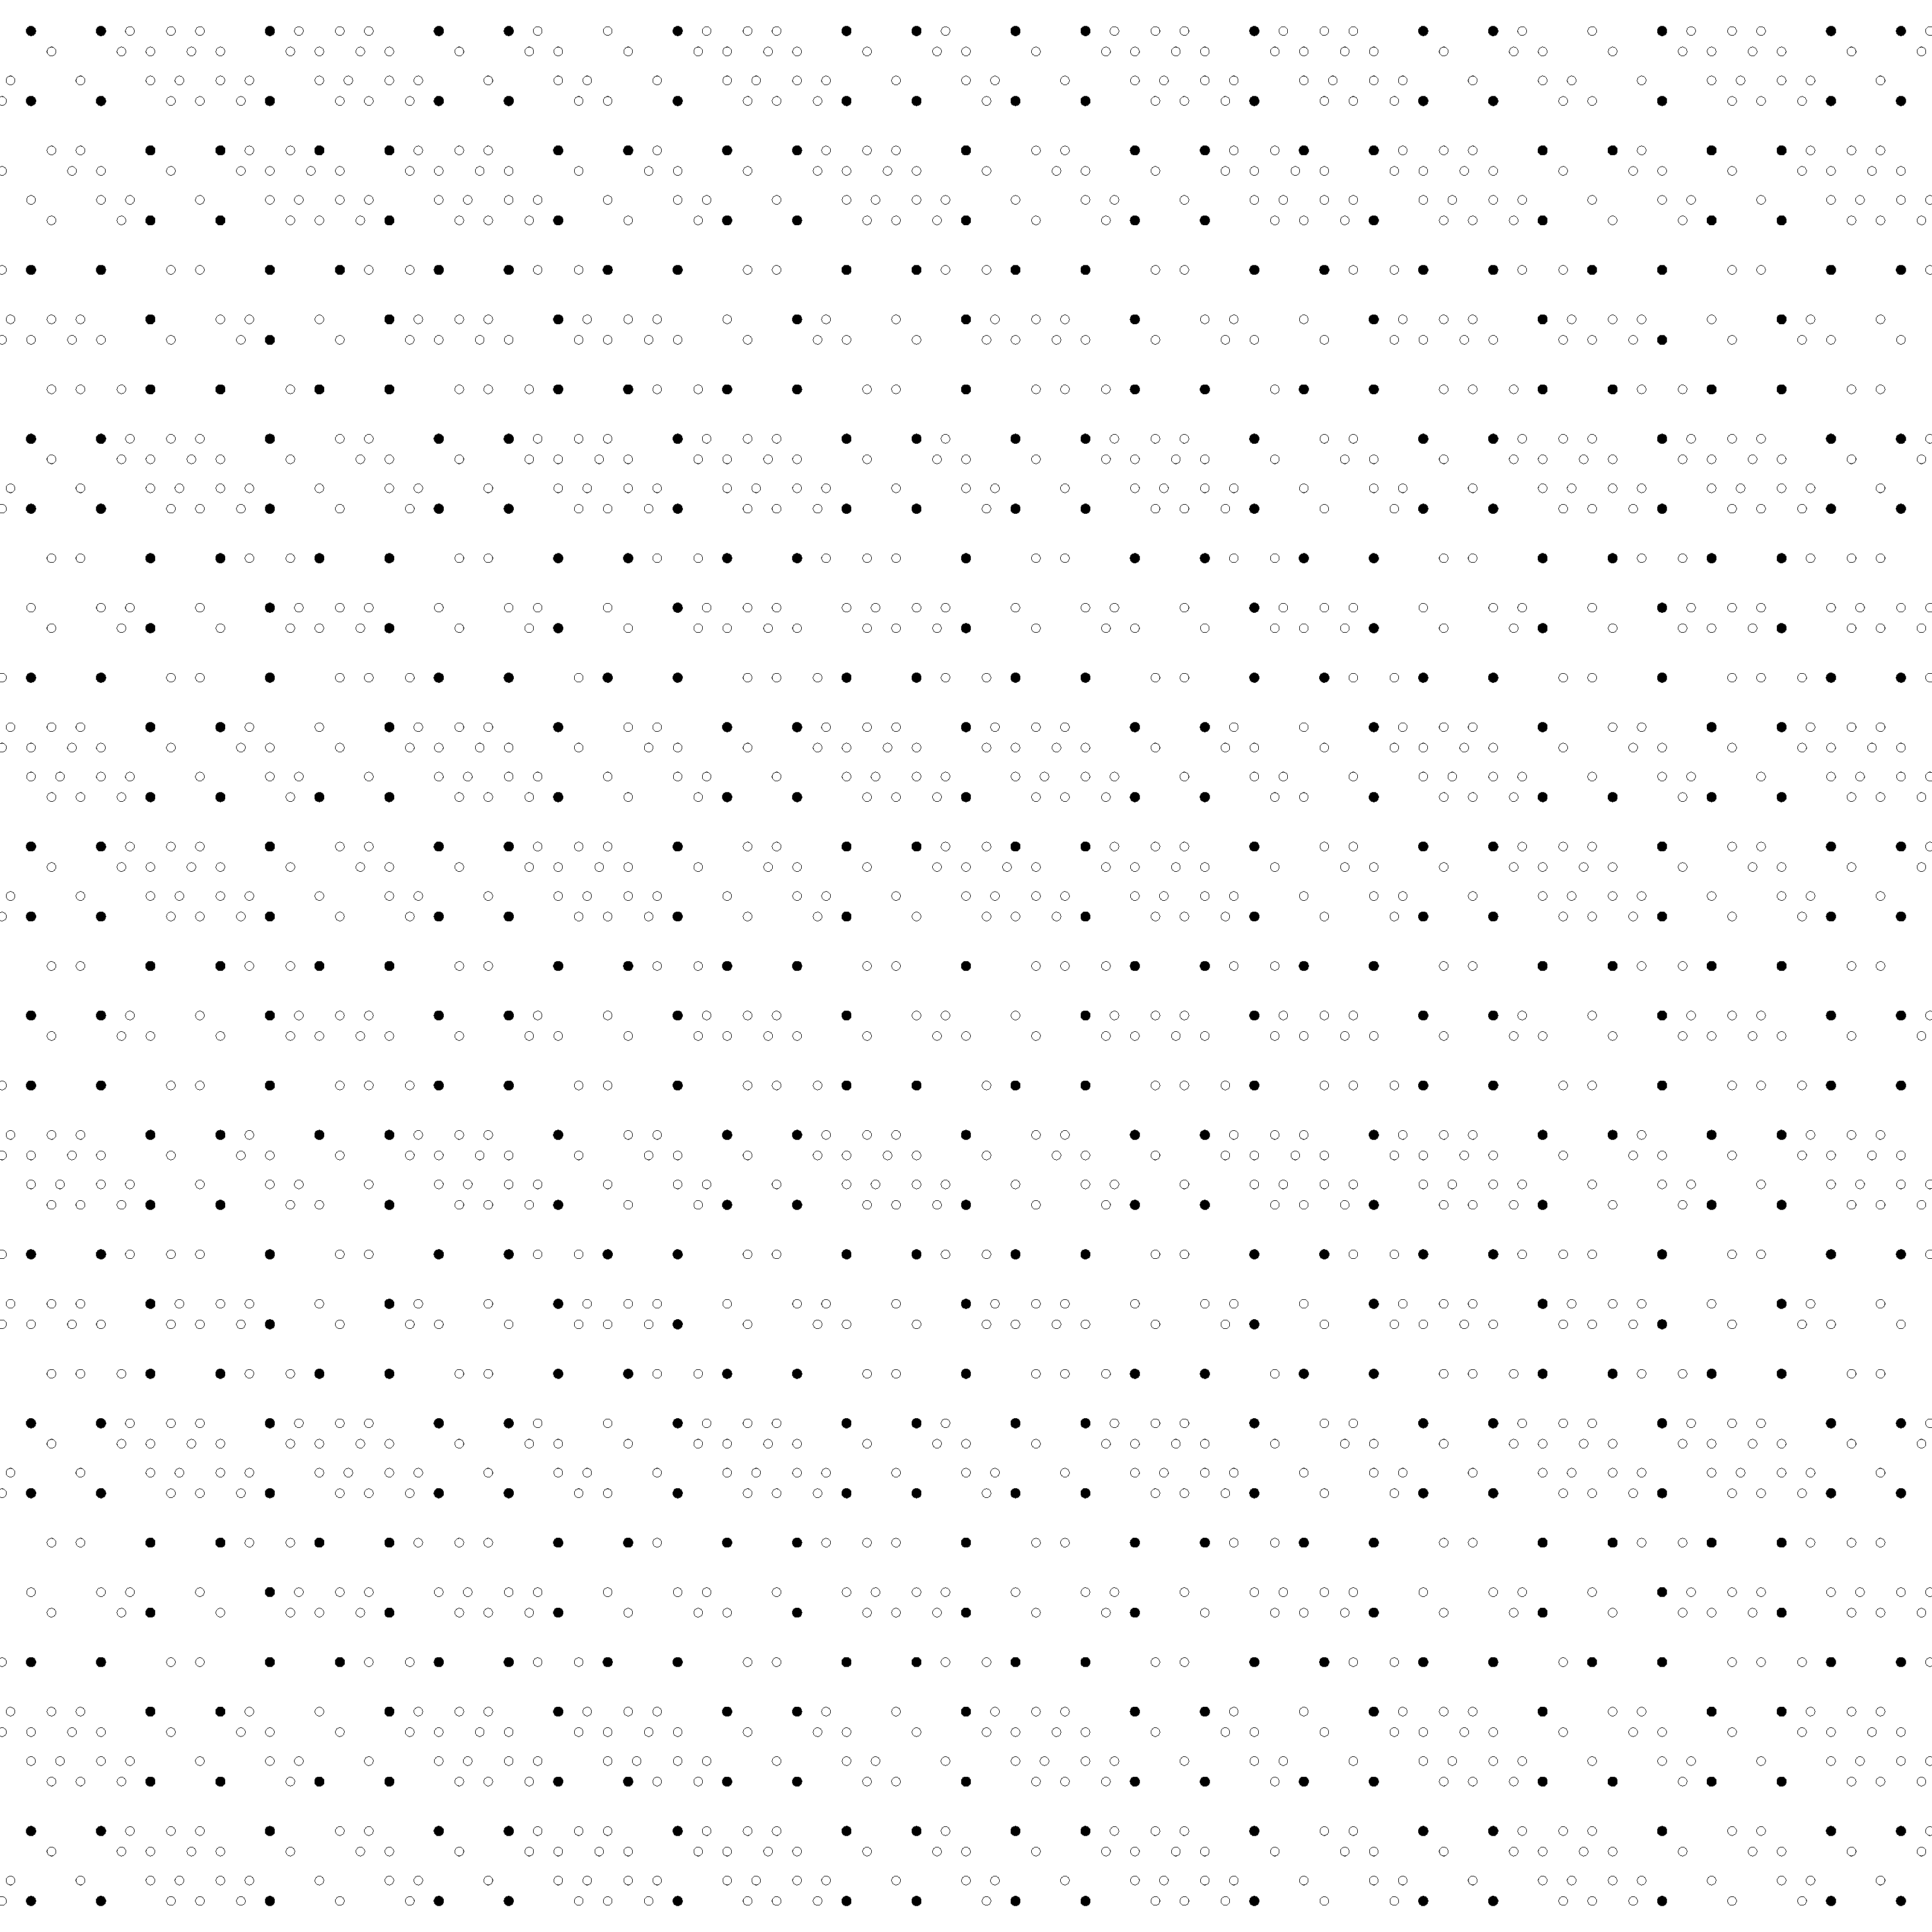
\includegraphics[width=0.9\textwidth]{img/2D/octagon}
\caption{Example of a finite section of a two dimensional quasicrystal with an octagonal window for Pisot-cyclotomic $\beta_8=1+\sqrt{2}$. The $\bullet$ points are the points of the quasicrystal with octagonal window and the $\circ$ and $\bullet$ points are points of the quasicrystal with a rhombic window circumscribed to the octagonal window. (Figure \ref{fig_quasicrystalExampleRhombus})}
\label{fig_quasicrystalExampleOctagon}
\end{figure}

To summarize, we are able to acquire a finite section of a quasicrystal with a rhombic window by composing two finite sections of a quasicrystal with one dimensional window. Through a finite section of a quasicrystal with a rhombic window we are able to acquire a finite section of a quasicrystal with any other window thanks to the inclusion property. 

\subsection{Estimate covering radius of the quasicrystal $R_C$}
There is much to gain from a proper covering radius estimate since it can greatly reduce the number of cases considered in the next step. We have tried several different ways to acquire the estimate. The method we present here worked the best for us. 

As a reminder here is the covering radius definition, simplified for two dimensions:\\
The \textbf{covering radius} of a set $D\subset \RR^2$ is the number: 
$$R_C = \inf\left\{ r_2>0\,\left|\, \forall\, z\in\RR^2:\; B(z,r_2)\cap D \neq \emptyset \right. \right\}$$

By Theorem \ref{the_voronoiCoveringRadius} we also have a way to calculate the covering radius from a Voronoi diagram:
$$R_C = \sup_{x\in D}\left\{\sup_{y\in V(x)}\lVert y-x\rVert\right\}$$

Here we run in a bit of a problem. The formula we suggested requires the list of Voronoi tiles that we do not know yet. In fact we want to use the covering radius estimate to acquire the list of Voronoi tiles. Luckily, there is a workaround. We do not actually need the complete list of Voronoi tiles to use the formula, just the one Voronoi tile that has the largest radius. There is a way to ensure we have the one tile without knowing the complete list of Voronoi tiles. 

First we need a way to acquire even an incomplete list of Voronoi tiles. We construct a Voronoi diagram of a finite section of the quasicrystal (described in previous step). That will result in possibly incomplete list of Voronoi tiles, the completeness depends on the size of the finite section. 

Now we need to make sure our possibly incomplete list of Voronoi tiles contains the one Voronoi tile with the largest radius. There is a way to show that any Voronoi tile that might be missing has smaller radius than at least one Voronoi tile already on the list. We recall the analysis of quasicrystals with one dimensional windows. There we have divided a window into sections corresponding to various Voronoi tiles. We can create the division of the window even with an incomplete list of Voronoi tiles. If the union of the sections $\Omega|_V$ is the entire window $\Omega$, our list of Voronoi tiles is sufficient for covering radius estimation. Now we look at this idea in greater detail. 

Assume a list of Voronoi tiles $\{V_1,\dots,V_m\}$, that may be incomplete. For each of the Voronoi tiles with domains $D_i = \{q_{i,1},\dots,q_{i,k_i}\}$ construct the following intersection: 
$$\Omega|_{V_i} = \bigcap\limits_{j\in\hat{k_i}}(\Omega-q_{i,j}^\ast)\cap\Omega$$

\begin{figure}[h!]
\centering
\begin{minipage}{0.25\textwidth}
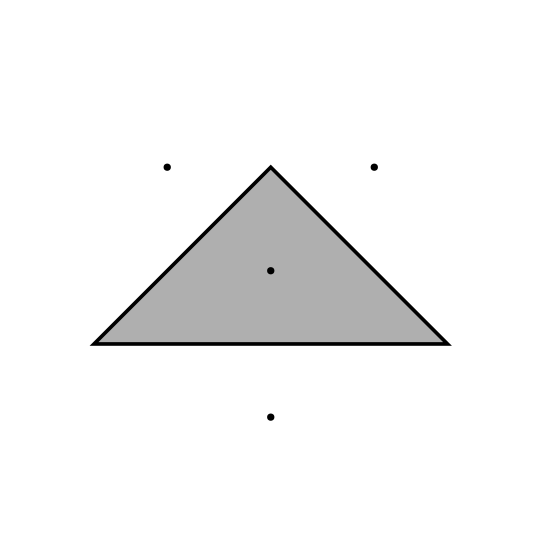
\includegraphics[width=\textwidth]{img/2D/intersectionTile01}
\end{minipage}
\qquad$\longmapsto$\qquad
\begin{minipage}{0.4\textwidth}
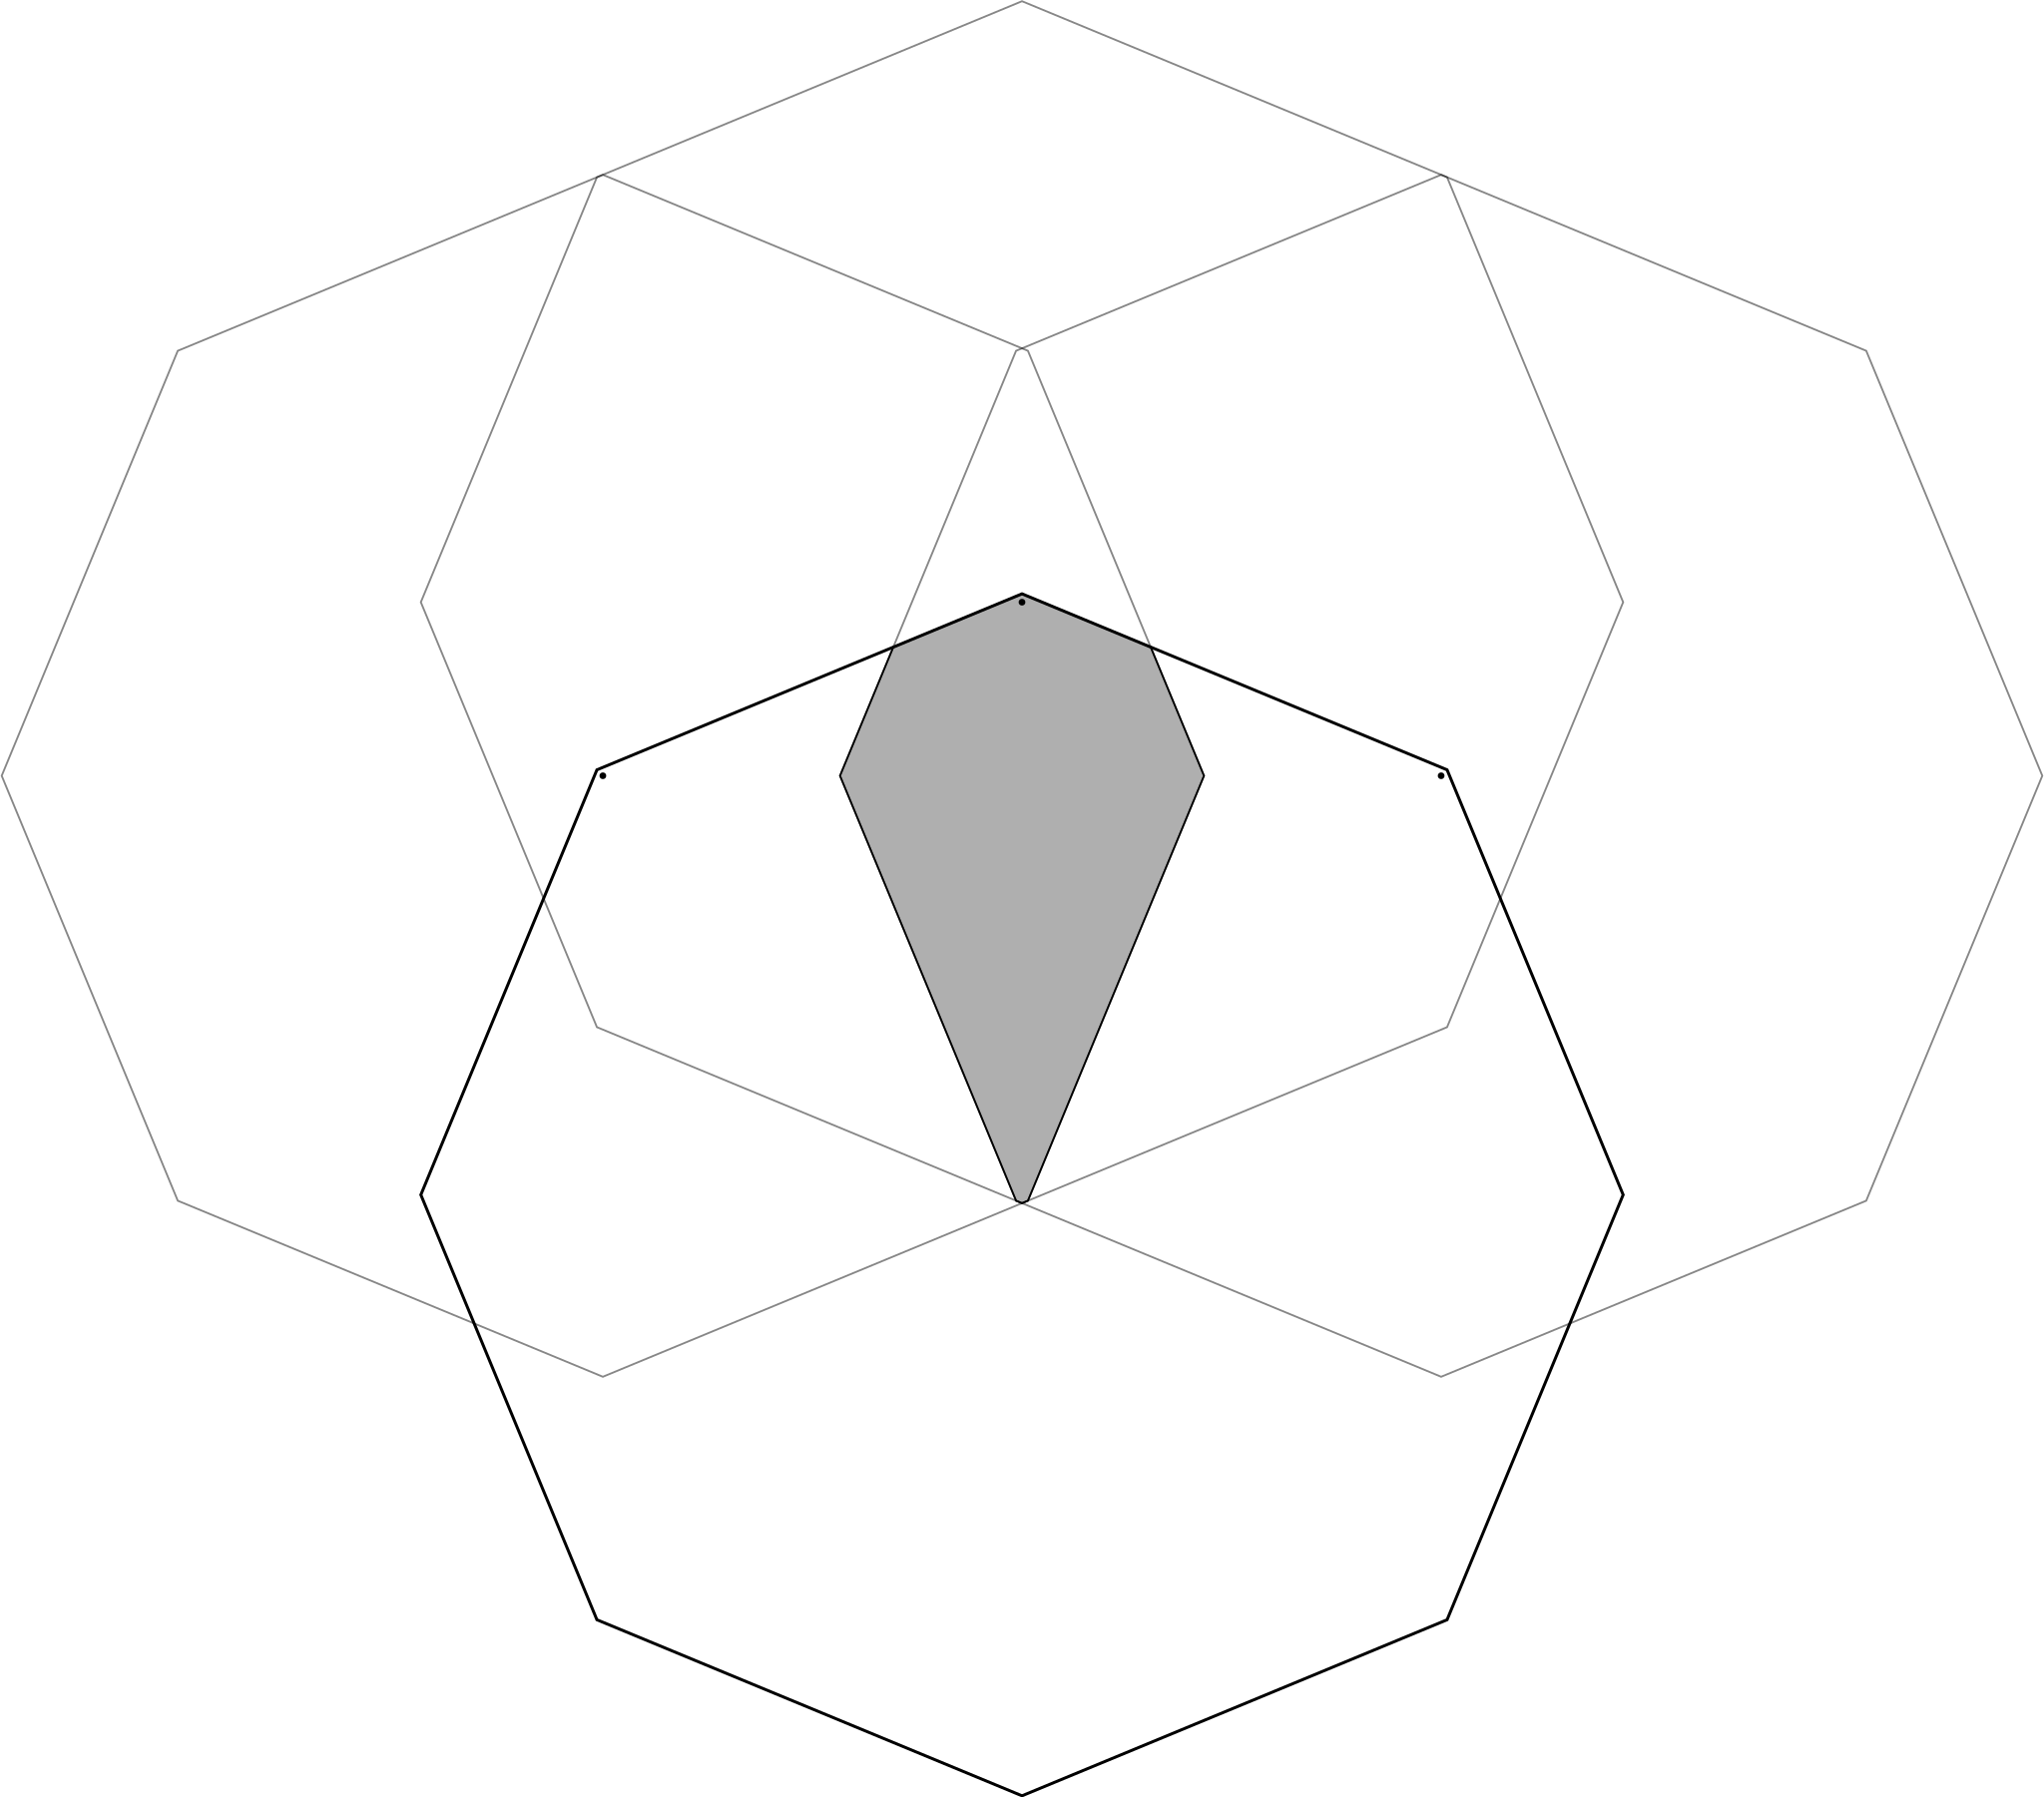
\includegraphics[width=\textwidth]{img/2D/intersection01}
\end{minipage}
\\[0.4cm]
\begin{minipage}{0.25\textwidth}
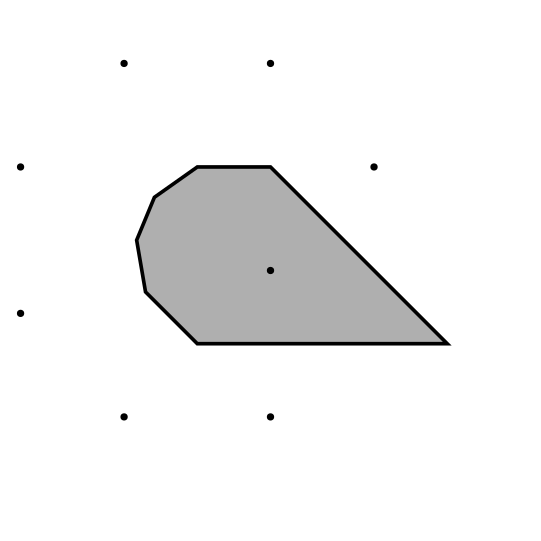
\includegraphics[width=\textwidth]{img/2D/intersectionTile02}
\end{minipage}
\qquad$\longmapsto$\qquad
\begin{minipage}{0.4\textwidth}
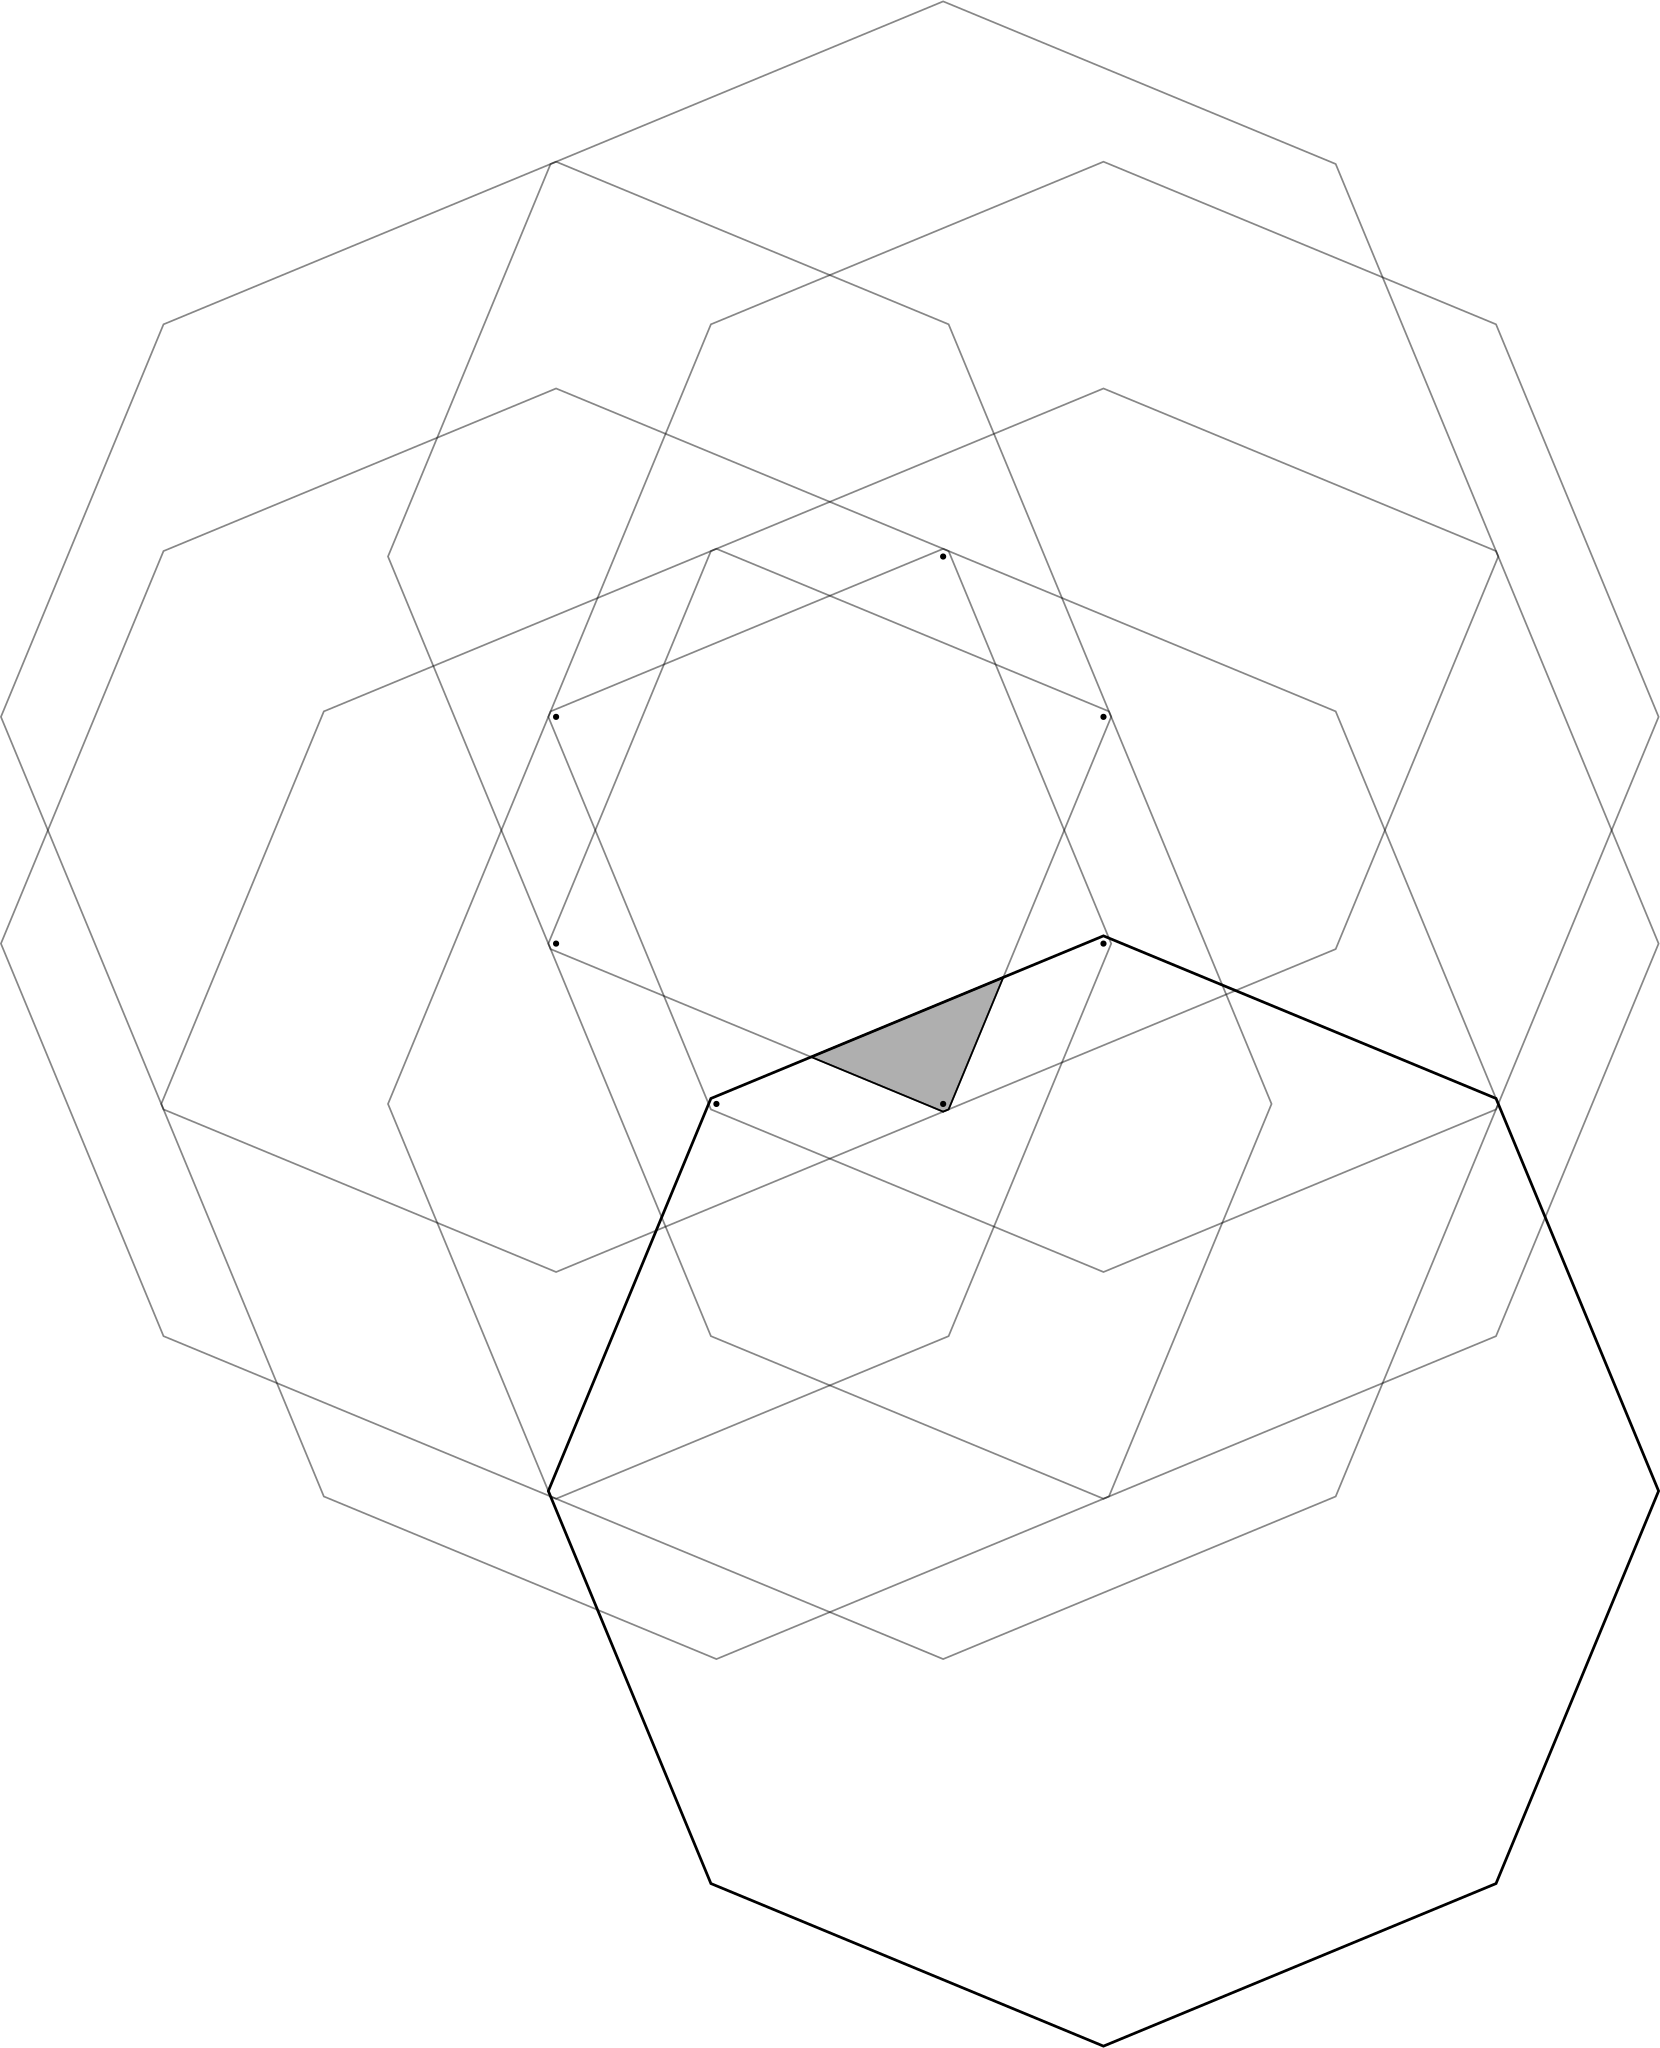
\includegraphics[width=\textwidth]{img/2D/intersection02}
\end{minipage}
\caption{Example of window intersectios for two Voronoi tiles. }
\label{fig_quasicrystalExampleIntersection}
\end{figure}

As we have discussed previously a point of the quasicrystal whose star map image fits in one of these intersections is surrounded by the corresponding domain. If several of these intersections overlap, a point whose star map image fits in the intersection of the intersections is surrounded by several domains. 

Once our list of Voronoi tiles $\{V_1,\dots,V_m\}$ covers the window by its intersections: 
$$\Omega = \bigcup\limits_{i\in\hat{m}}\Omega|_{V_i}$$
any missing Voronoi tile's intersections would overlap the current ones and thus the missing Voronoi tile would have a smaller radius. 

\begin{figure}[h!]
\centering
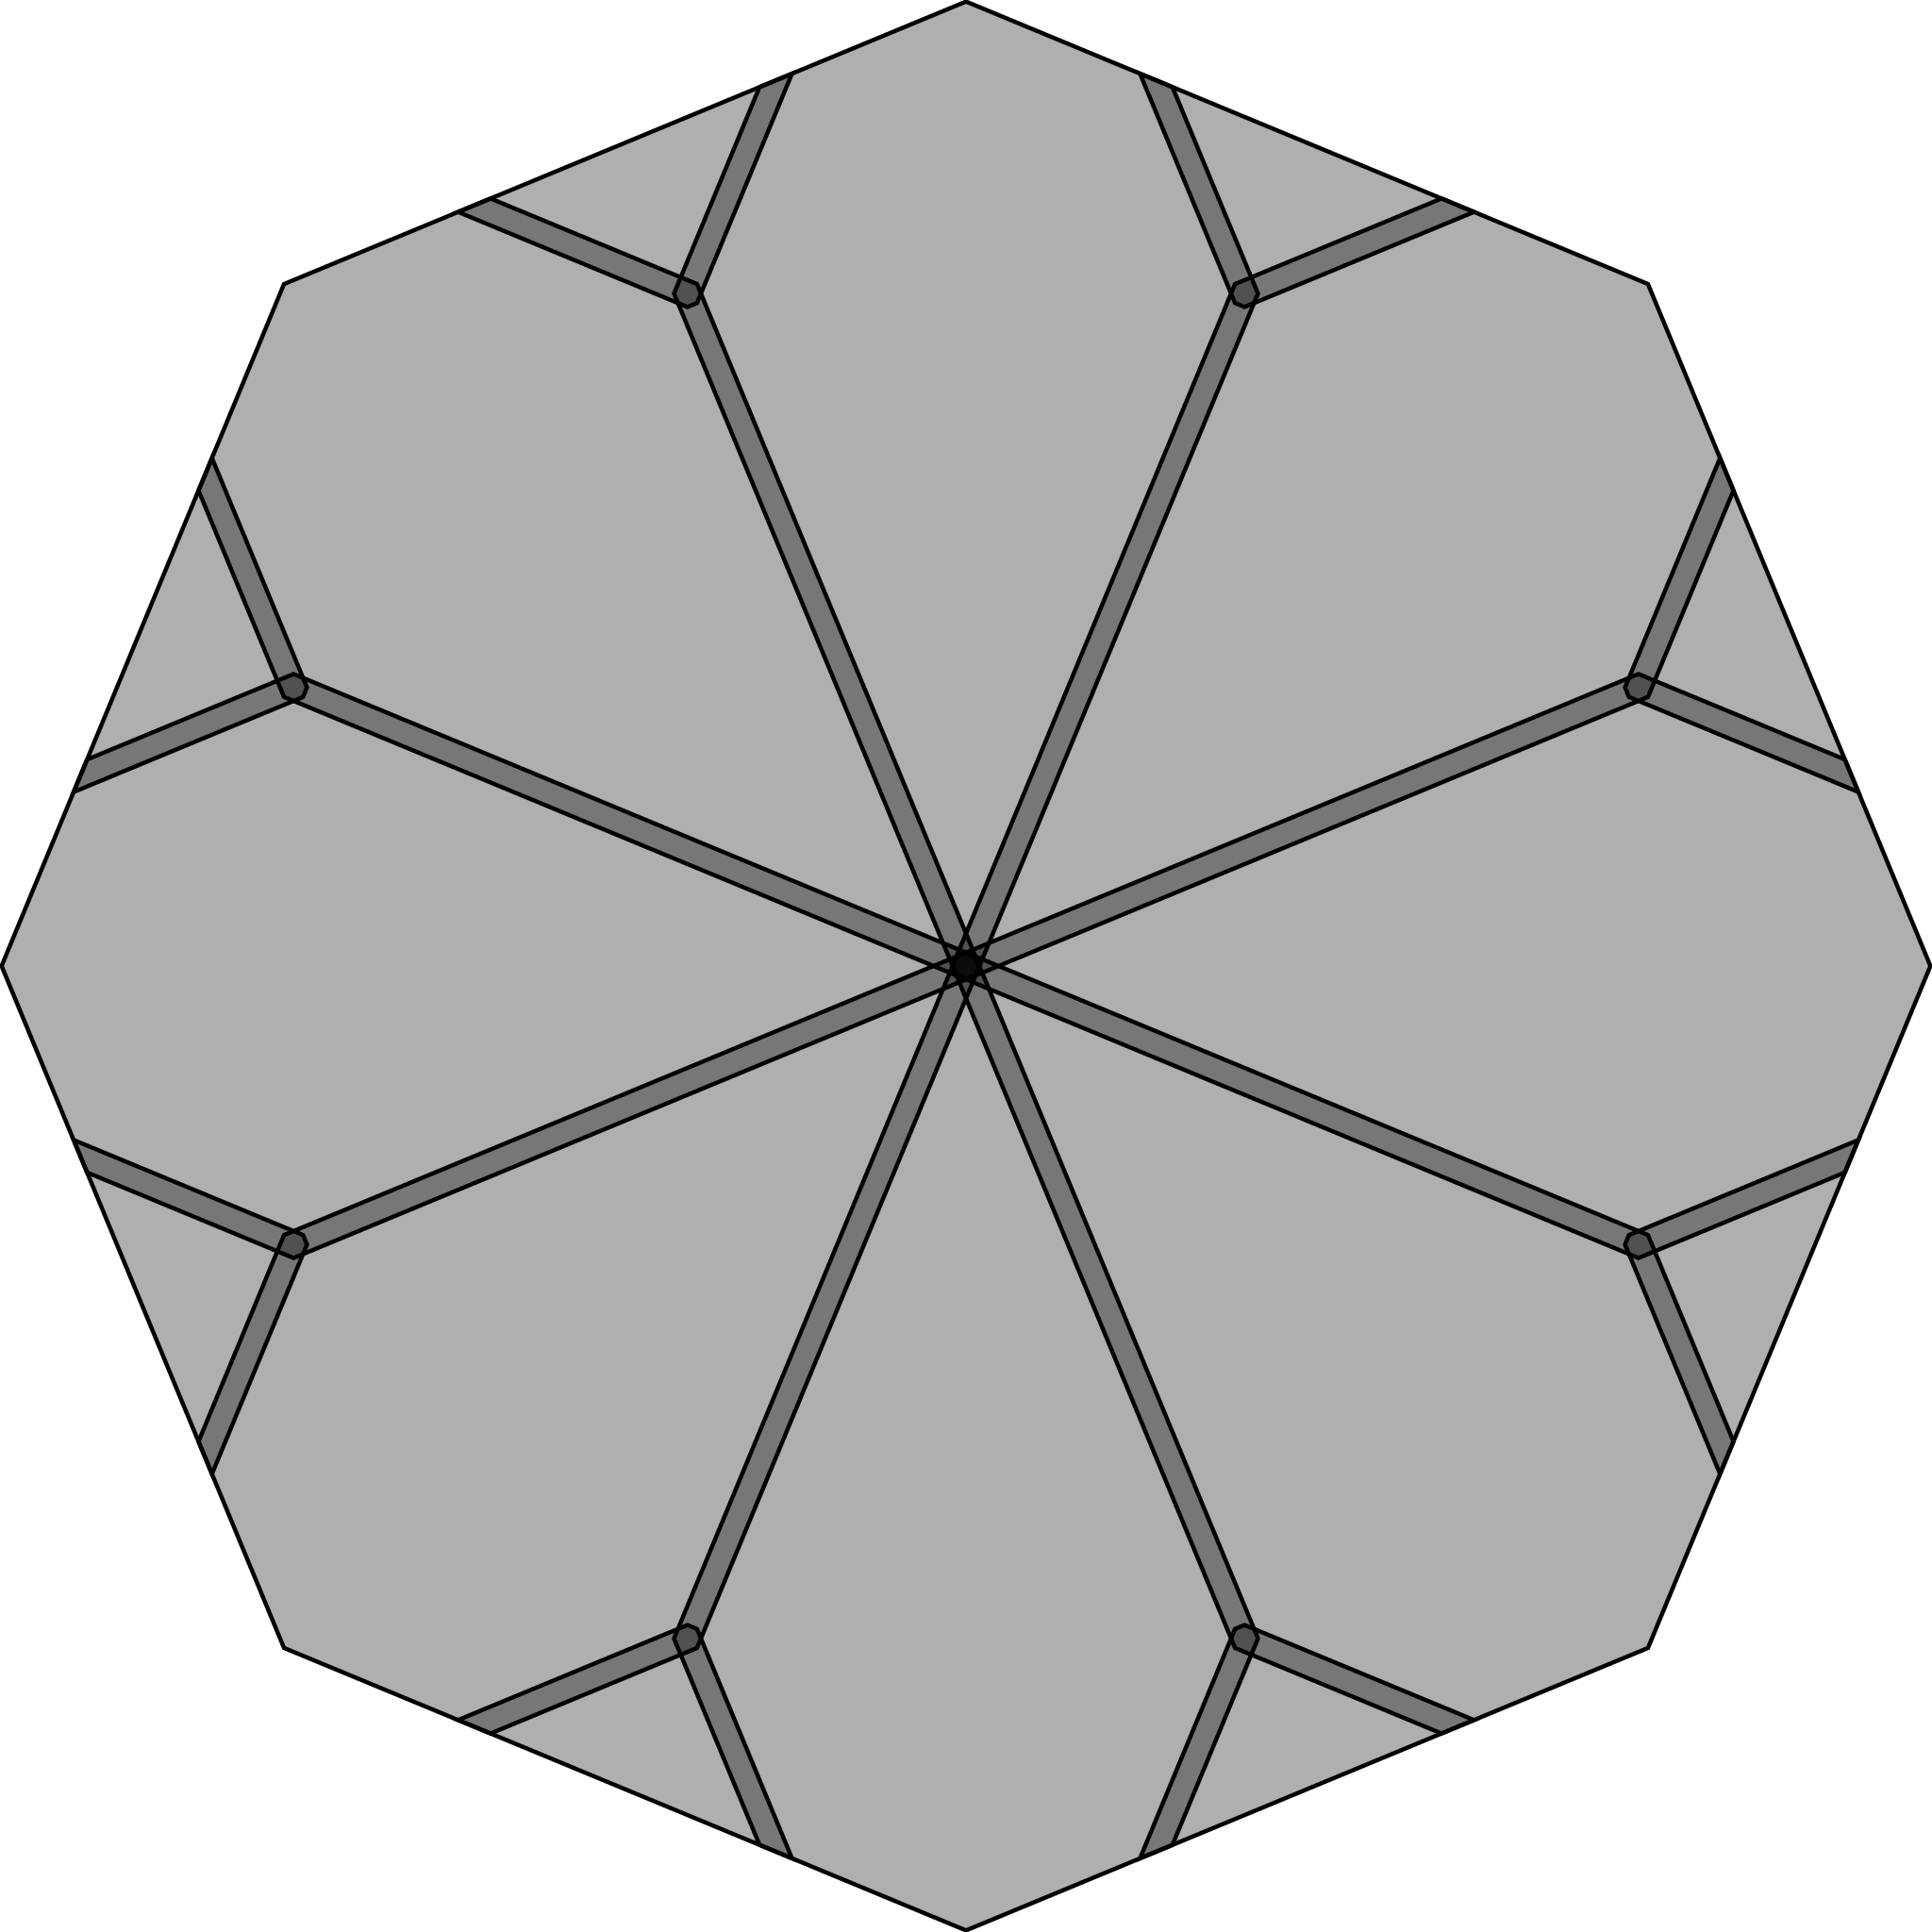
\includegraphics[width=0.4\textwidth]{img/2D/cover}
\caption{Example of a octagonal window covered by intersections of only sixteen Voronoi tiles including the two from Figure \ref{fig_quasicrystalExampleIntersection} (there are many more in the quasicrystal). }
\label{fig_quasicrystalExampleOctagonWindow}
\end{figure}

\begin{figure}[h!]
\centering
\begin{minipage}{0.25\textwidth}
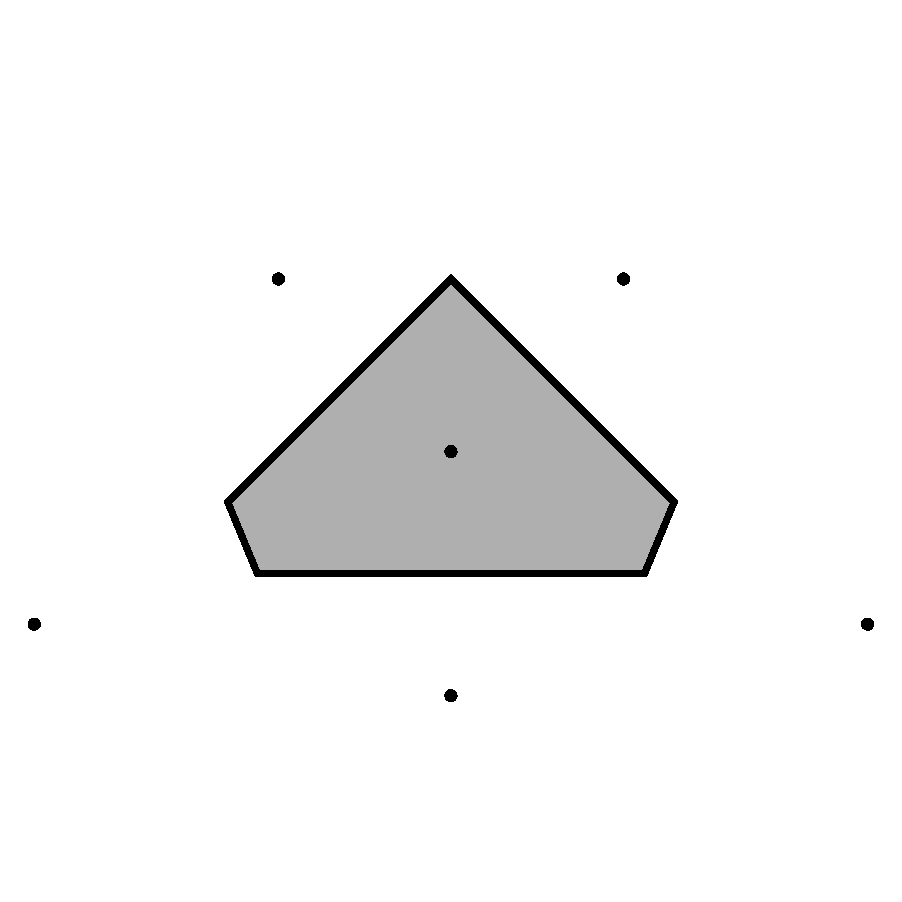
\includegraphics[width=\textwidth]{img/2D/intersectionTile03}
\end{minipage}
\qquad$\longmapsto$\qquad
\begin{minipage}{0.4\textwidth}
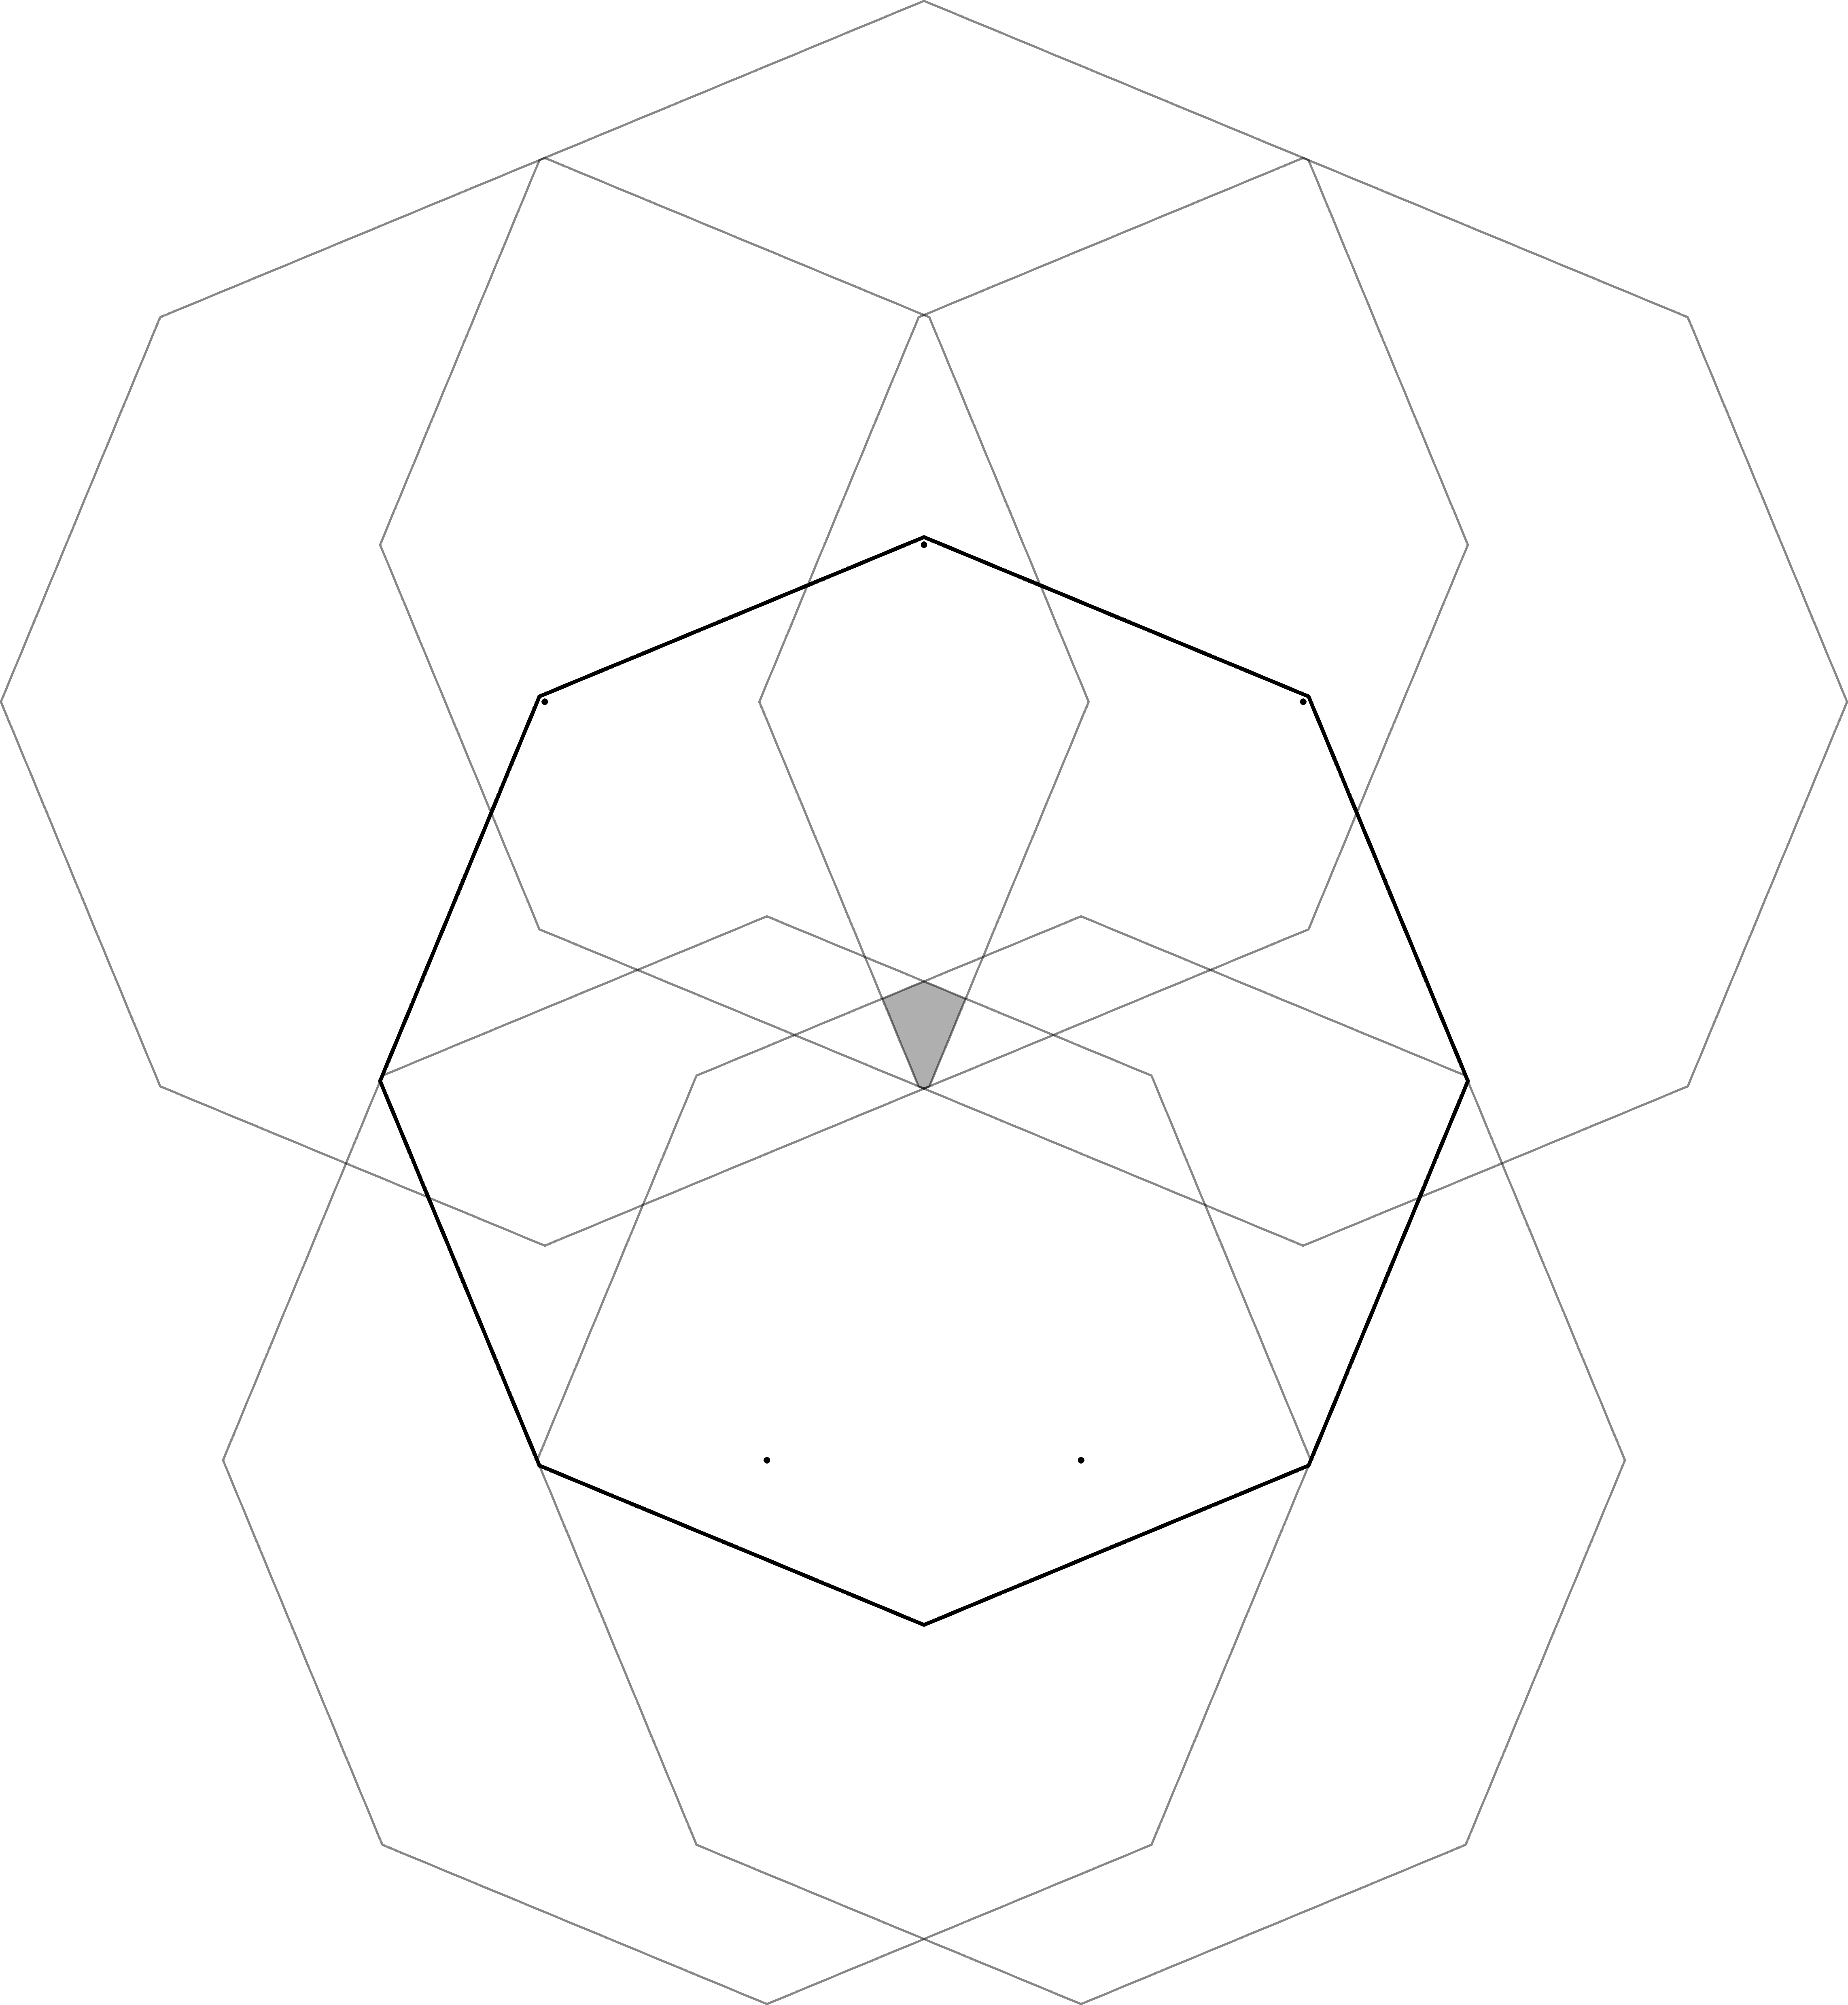
\includegraphics[width=\textwidth]{img/2D/intersection03}
\end{minipage}
\caption{Example of a Voronoi tile whose intersection would overlap one of the intersections in Figure \ref{fig_quasicrystalExampleOctagonWindow} and it indeed has smaller radius than the two considered Voronoi tiles in Figure \ref{fig_quasicrystalExampleIntersection}. }
\label{fig_quasicrystalExampleIntersection02}
\end{figure}

To summarize, assume a list of Voronoi tiles $\{V_1,\dots,V_m\}$, that may be incomplete, with domains $D_i = \{q_{i,1},\dots,q_{i,k_i}\}$. Then given another condition the estimate $\hat{R}_C$ of covering radius $R_C$ is obtained as:
$$\Omega = \bigcup\limits_{i\in\hat{m}}\Omega|_{V_i} \qquad\Rightarrow\qquad \hat{R}_C \overset{\text{def}}{=} R_C = \max_{i\in\hat{m}}\left\{\sup_{y\in V_i}\lVert y\rVert\right\}$$

The series of articles \cite{classification}, \cite{classificationII} and \cite{classificationIII} that our work is based upon, used an easier method for covering radius estimation that results in a worse estimate than the method we have just described. Since the quasicrystals we are analyzing have higher complexity, improving the covering radius estimate in this way was absolutely vital to progress in our analysis. 

\subsection{Generate superset of all finite sections spanning $B(2\hat{R}_C)$}\label{sec_2DsupersetFiniteSections}
This step is also solved by the rhombus decomposition and the inclusion property. Previously we have developed an algorithm to acquire all possible finite sections of a quasicrystal with one dimensional window spanning a given length. If we compose each pair of these into finite sections of a quasicrystal with rhombic window, we acquire a list of all possible finite sections spanning a rhombic area. Thus the length given to the algorithm to acquire all possible finite sections of a quasicrystal with one dimensional window must be the length of an edge of a rhombus circumscribed to $B(2\hat{R}_C)$. 

Finding a formula to calculate the length of an edge of the rhombus $a$ circumscribed to $B(2\hat{R}_C)$ from $\hat{R}_C$ is just a trigonometric exercise and we will not cover it here. The formula is: 
$$a^2 = \frac{16\hat{R}_C^2}{\left(1+\frac{\rho}{2}\right)\left(1-\frac{\rho}{2}\right)}$$
where $\rho$ is the $\rho=2\cos\left(2\pi/n\right)$ to which $\beta$ is associated. 

Once we calculate $a$ we can acquire all possible finite sections of a quasicrystal with one dimensional window spanning $a$ and then for each pair compose a finite section of the quasicrystal with the rhombic window. Of course we can also crop these by $B(2\hat{R}_C)$. 

\begin{figure}[h!]
\centering
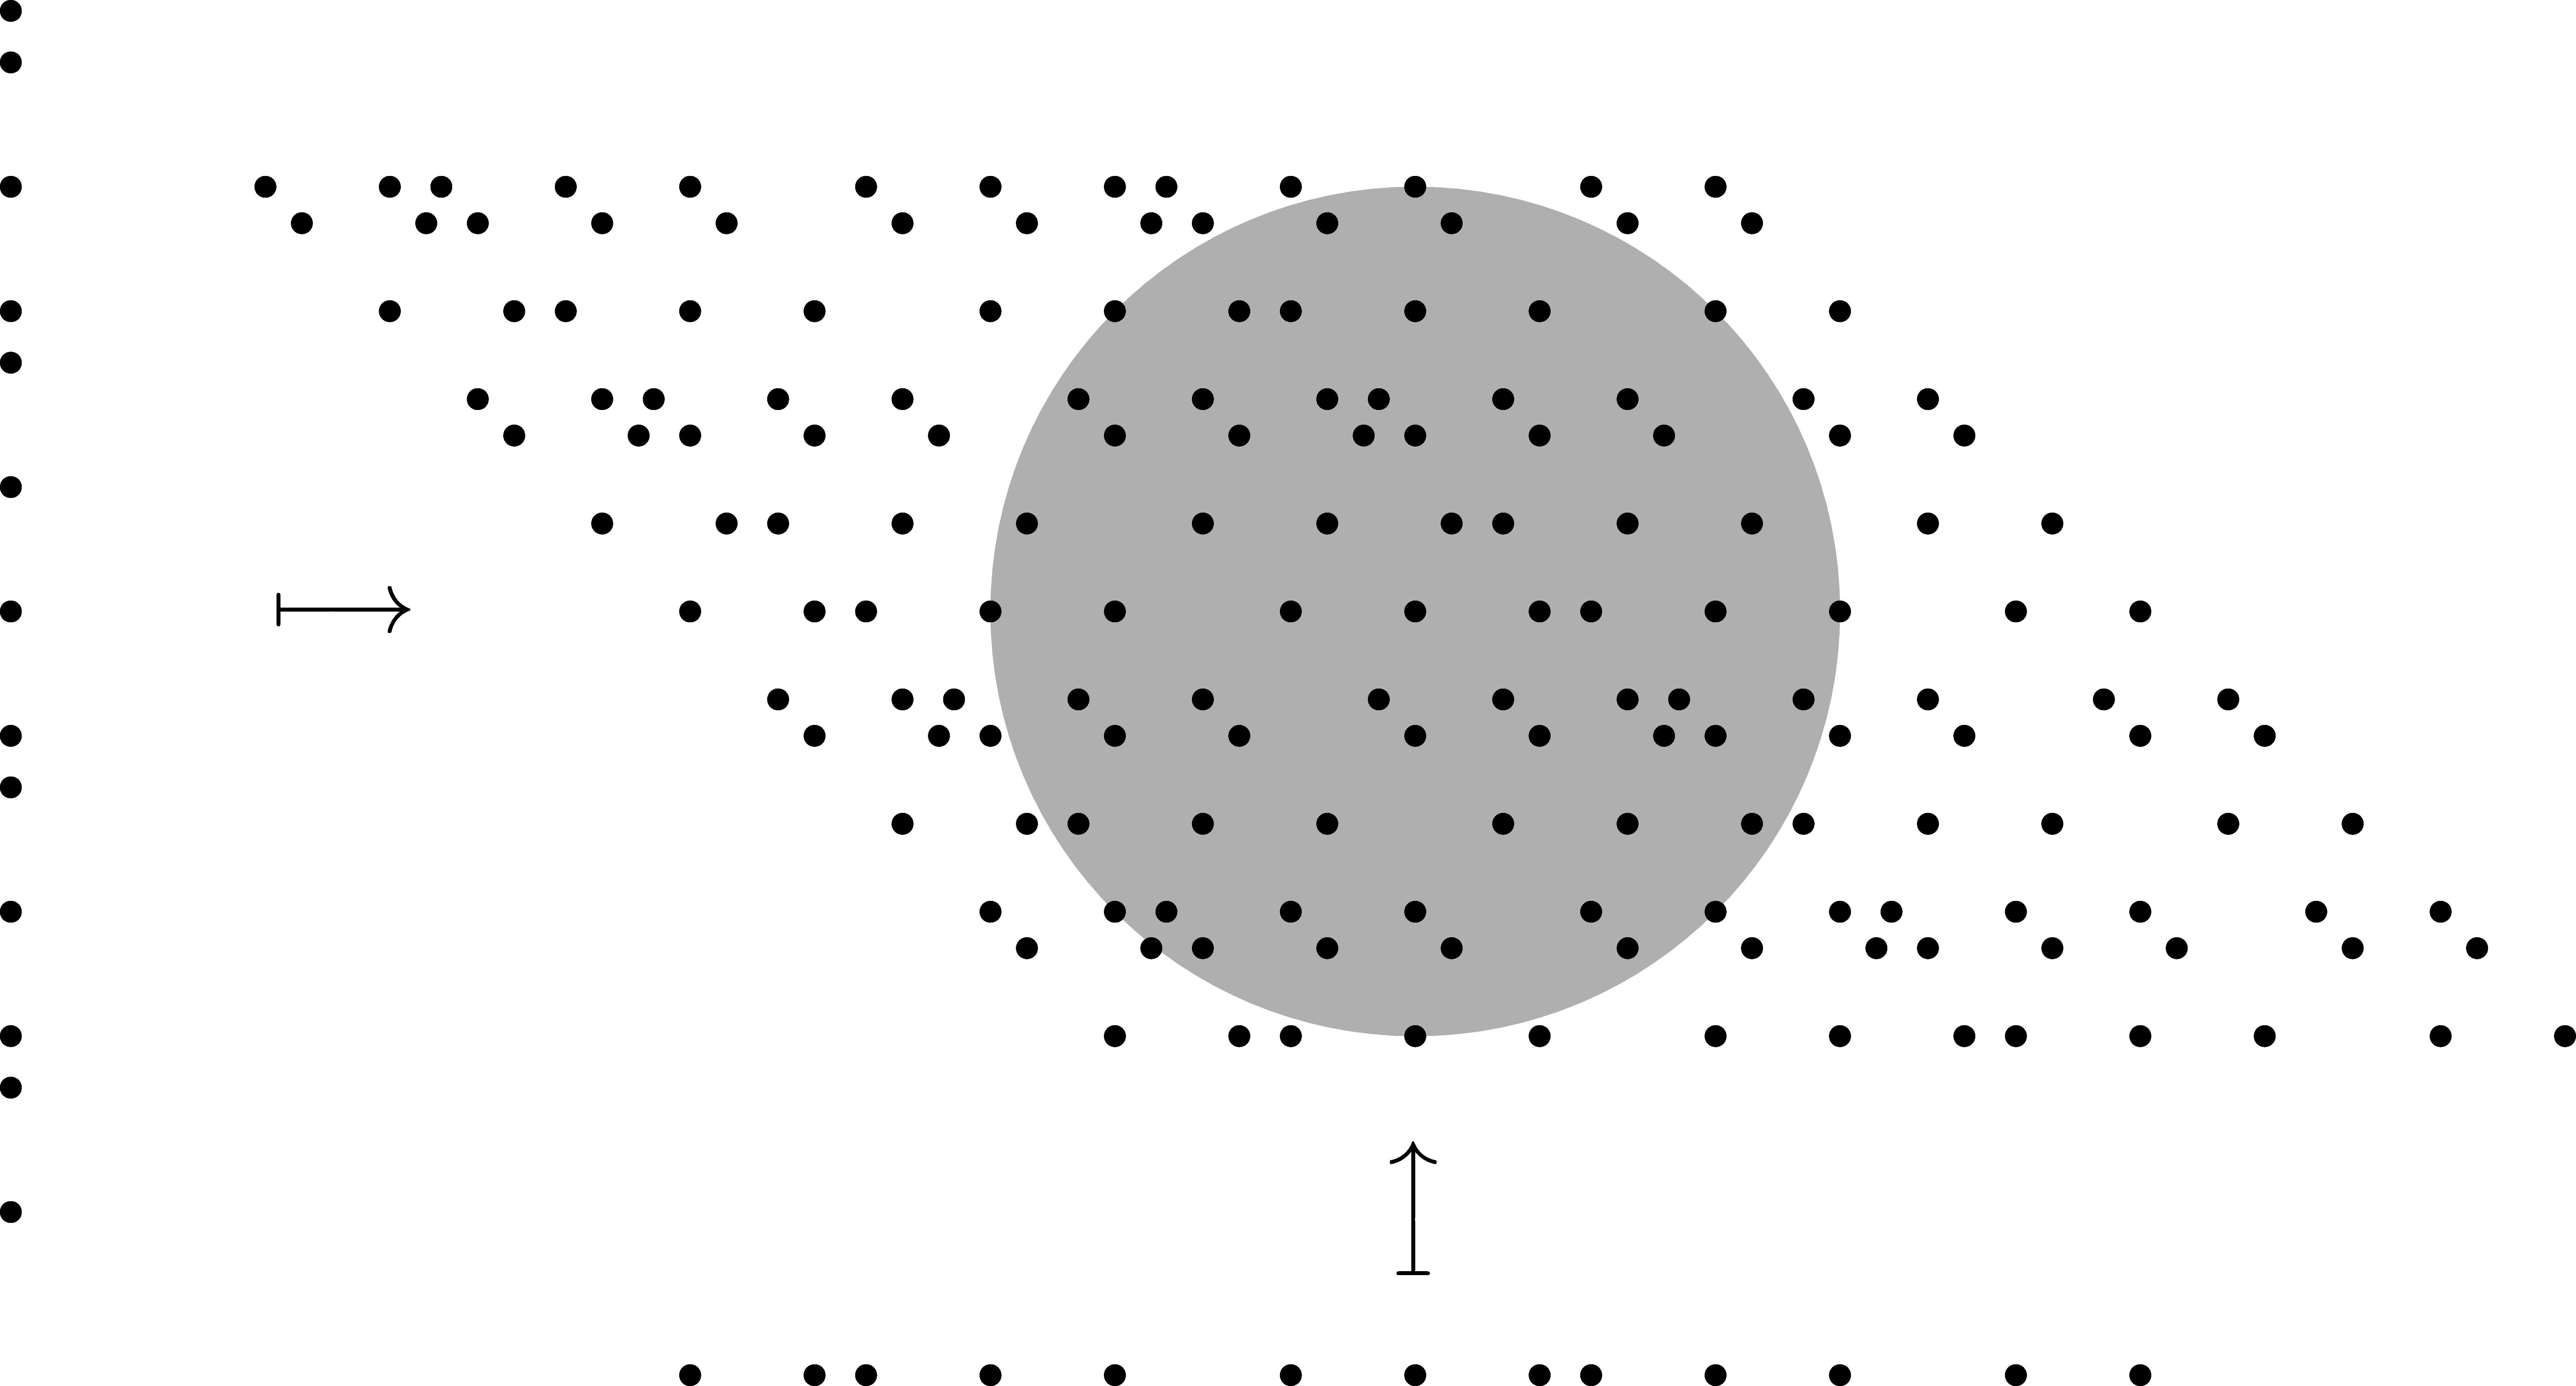
\includegraphics[width=0.7\textwidth]{img/2D/compositionFinite}
\caption{Example of the composition of a finite section of a quasicrystal with a rhombic window from two finite section of a quasicrystal with one dimensional window. The circle has radius $2\hat{R}_C$. }
\label{fig_quasicrystalExampleComposition}
\end{figure}

That completes the task of acquiring a list of all possible finite sections of a qusicrystal with a rhombic window, the easy part of this step. Now we have to use the inclusion property to somehow turn this list of all possible finite sections of a qusicrystal with a rhombic window to a list of all possible finite sections of a qusicrystal with any window. 

We cannot use the same method we used in the first step of this analysis since the finite sections are centered around the origin, whereas in the actual quasicrystal they may be almost arbitrarily translated. 

The inclusion property only tells us that there can be no more points in the finite sections of the quasicrystal with any window inscribed to a rhombic window than in the finite sections of the quasicrystal with the rhombic window. 

Naive approach to solving this would be to treat each point in each finite section of the quasicrystal with the rhombic window as optional and create a superset exhausting all options. Such superset would contain all finite sections of the quasicrystal with any window inscribed to the rhombic window, which of course includes the window we are interested in. While this is true in theory, it is very impractical for actually acquiring the list of finite sections since such superset would be enormous. 

There again are many ways of solving this issue and we present the method that worked best for us. Our method slightly deviates from the course of our general quasicrystal analysis in that it does not generate a superset of all finite sections spanning $B(2\hat{R}_C)$ but rather a superset of all domains of Voronoi tiles that appear in the qusicrystal with the window we are interested in, that might but also might not be the same thing. 

Just as in the previous step we are going to use a possibly incomplete list of Voronoi tiles $\{V_1,\dots,V_m\}$, with domains $D_i = \{q_{i,1},\dots,q_{i,k_i}\}$, acquired by searching the Voronoi diagram of a finite section of the quasicrystal, that cover the window $\Omega$ by its intersections:
$$\Omega = \bigcup\limits_{i\in\hat{m}}\bigcap\limits_{j\in\hat{k}_i}(\Omega-q_{i,j}^\ast)\cap\Omega$$ 
Now assume a Voronoi tile $V$ with domain $D = \{q_1,\dots,q_k\}$ that appears in the quasicrystal but is missing from the list $\{V_1,\dots,V_m\}$. Its intersection $\bigcap_{j\in\hat{k}}(\Omega-q_j^\ast)\cap\Omega$ has to overlap with at least one intersection of a Voronoi tile on the list, let us denote this Voronoi tile as $V_p$. 

A point of the quasicrystal whose star map image fits both in the intersection of $V$ and the intersection of $V_p$ is surrounded by the points of $D$ as well as the points of $D_p$. In other words the Voronoi tile $V$  is a subset of $V_p$ and its domain $D$ is a subset of $D_p\cup F$, where $F$ is a finite section of the quasicrystal with the rhombic window. 

The algorithm should now be quite clear. For each $V_i\in\{V_1,\dots,V_m\}$ and for each finite section of the quasicrystal with the rhombic window we add points of the finite section to the domain $D_i$ and save the domain of any new Voronoi tile that is thusly created. As stated before, this creates a superset of domains of Voronoi tiles that appear in the quasicrystal. 

\begin{figure}[h!]
\centering
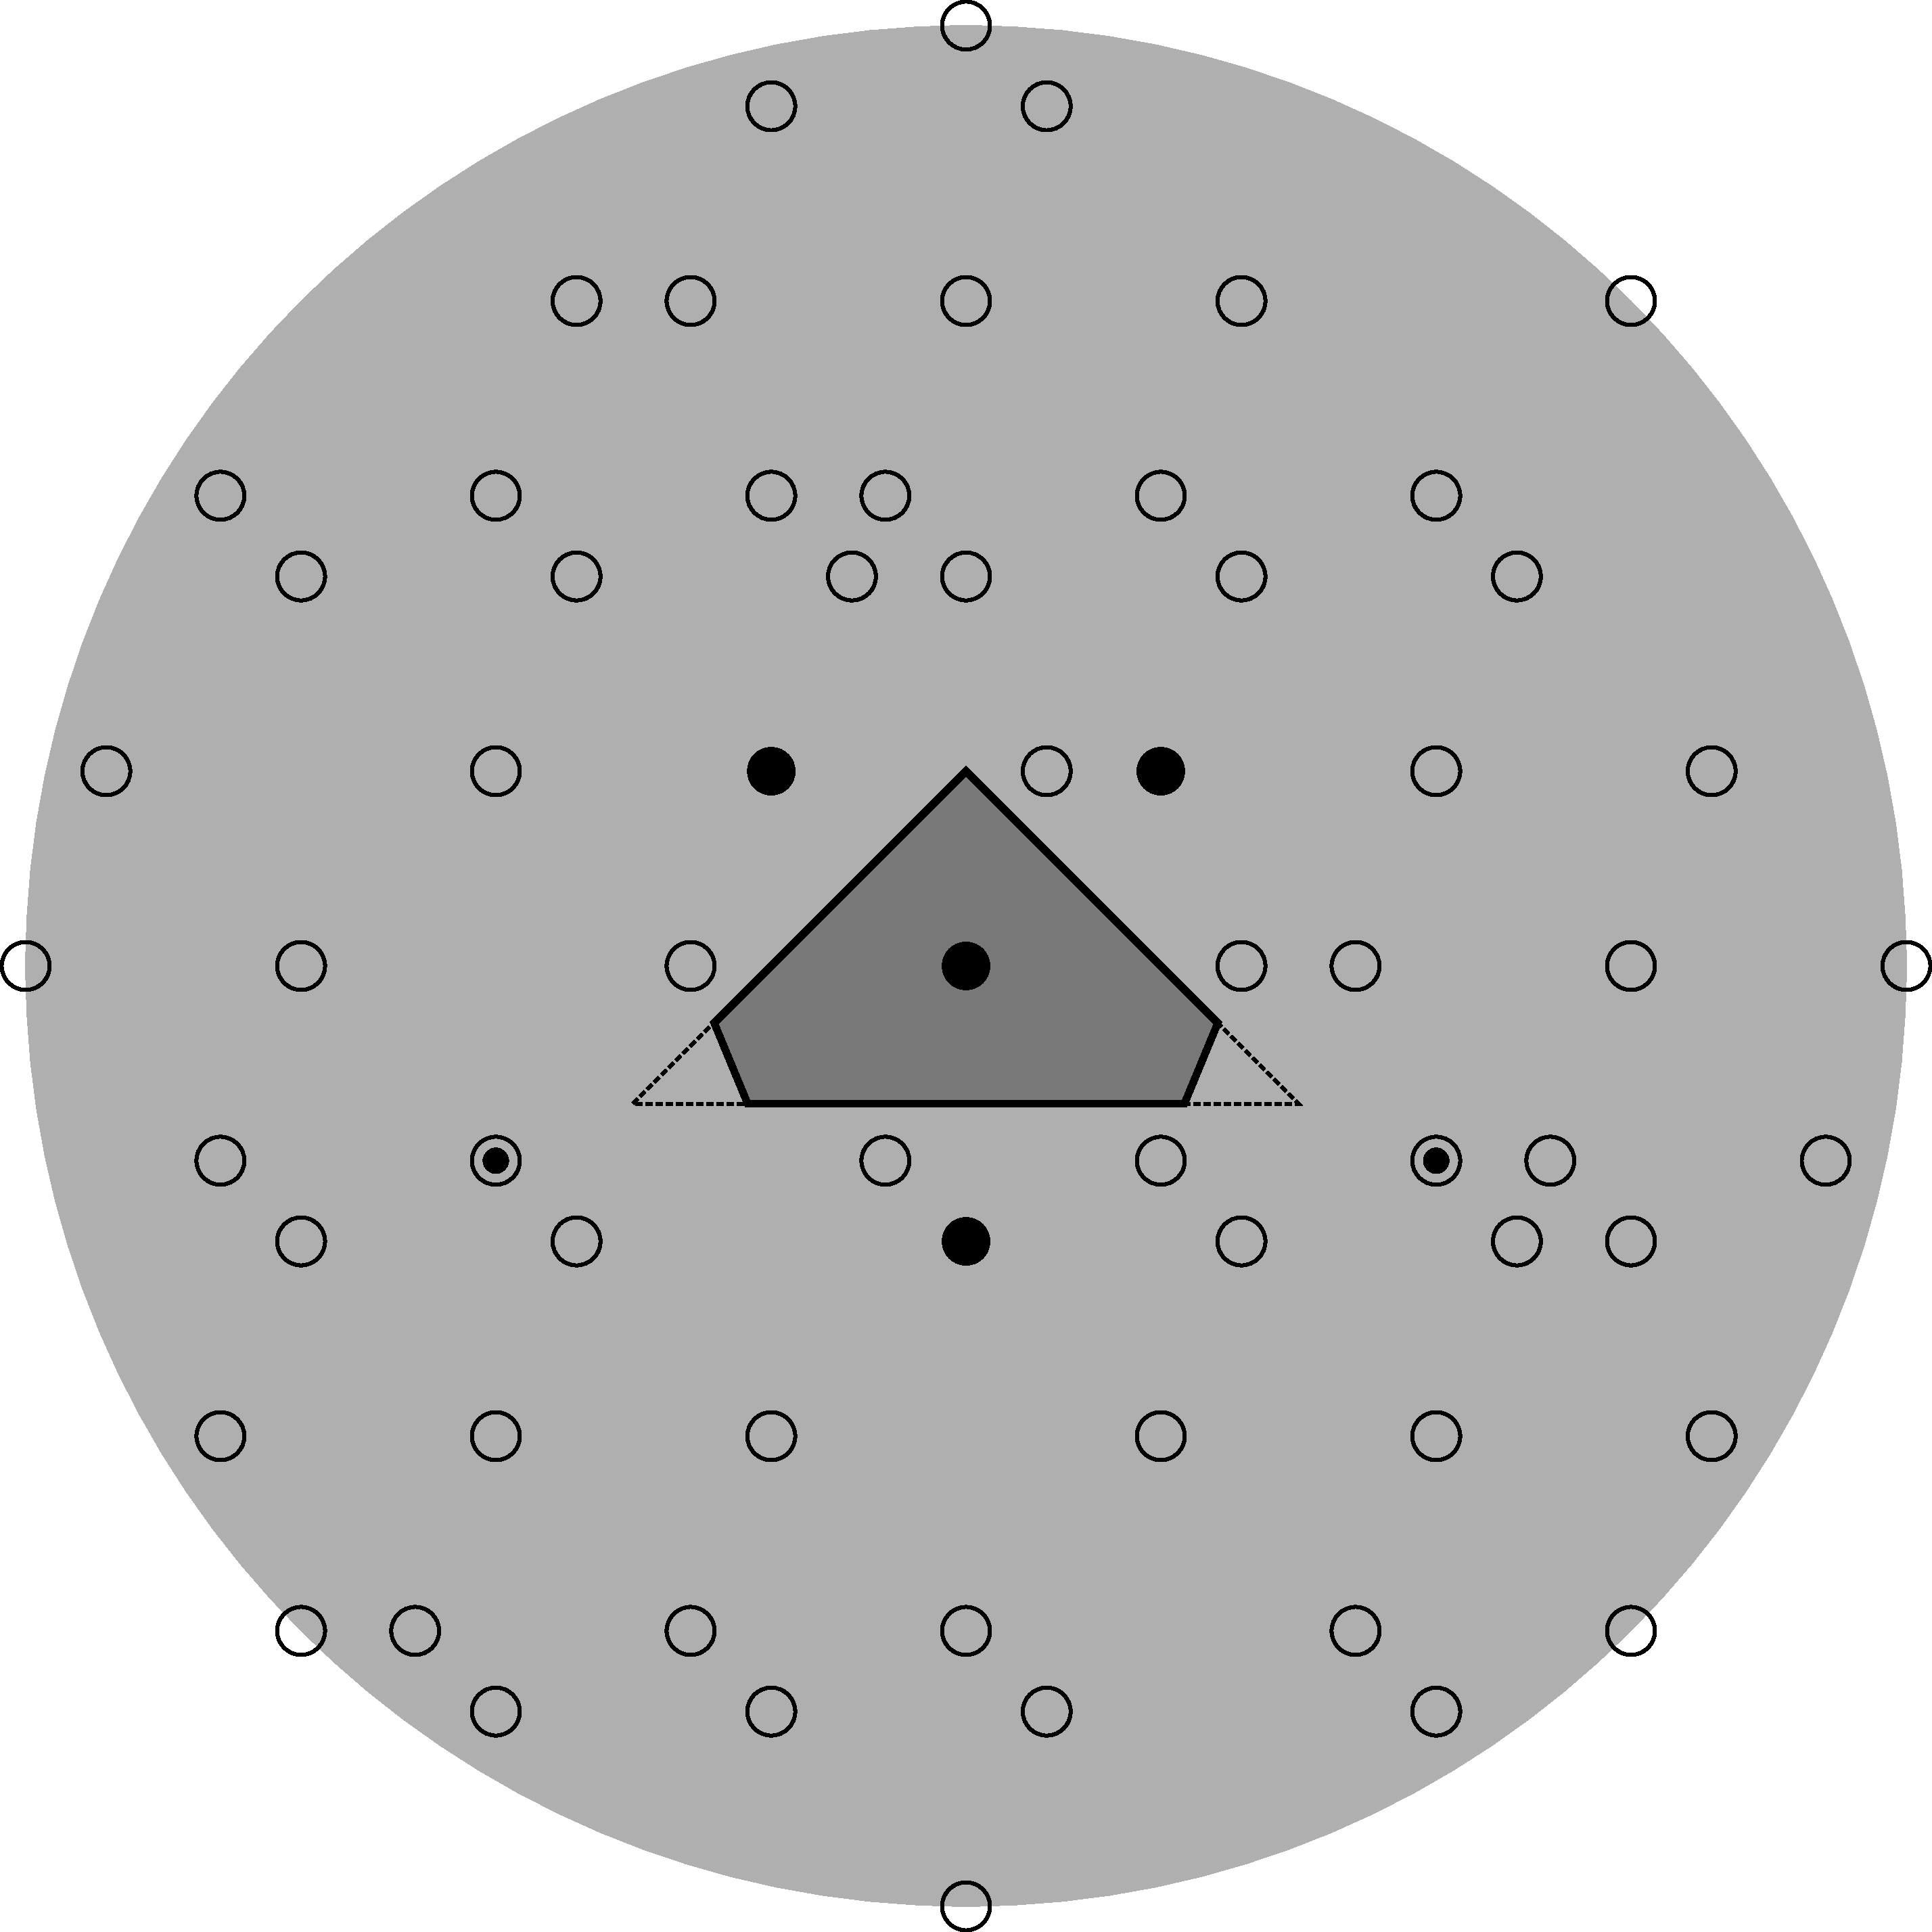
\includegraphics[width=0.4\textwidth]{img/2D/cropByFiniteSection}
\caption{Example of how a new Voronoi tile is created from the incomplete list of Voronoi tiles and the list of finite sections. The first Voronoi tile from Figure \ref{fig_quasicrystalExampleIntersection} and the finite section from Figure \ref{fig_quasicrystalExampleComposition} are used to create the Voronoi tile from Figure \ref{fig_quasicrystalExampleIntersection02} by adding two points $\odot$ of the finite section. }
\label{fig_quasicrystalExampleNewTile}
\end{figure}

\subsection{Filter the superset to the final list of Voronoi tiles}
This step is not at all different from what we did for the quasicrystal with one dimensional window. We follow the same three filters: 
\begin{enumerate}
\item Eliminate duplicate Voronoi tiles. 
\item Eliminate Voronoi tiles whose intersection $\Omega|_{V} = \bigcap\limits_{i\in\hat{k}}(\Omega-q_i^\ast)\cap\Omega$ is empty. 
\item Eliminate Voronoi tiles whose section $\Phi(V) = \Omega|_{V}\setminus\bigcup_{|U|<|V|}\Omega|_{U}$ is empty. 
\end{enumerate}

There might be a technical difficulty with verifying whether $\Phi(V)$ is empty. Here we again turn to the inclusion--exclusion principle we described in Section \ref{sec_1DperiodOfVoronoiTile}. 

Unlike with one dimensional quasicrystals where we have picked left-closed right-open interval to avoid configurations that appear only once in the entire quasicrystal (i.e.\ have zero density), here we simply cannot avoid zero density configurations. 

First let us explain what exactly are these zero density configurations and where do they come from. For a particular window $\Omega$ and a particular Voronoi tile $V$ it may happen that the intersection $\Omega|_V$ is just a single point. Such Voronoi tile would appear in the quasicrystal $\quasi{\Omega}$ only once. Additionally for the $n$-gonal window it may happen that a particular Voronoi tile has the intersection of a line segment. Such Voronoi tile would appear in the quasicrystal only countably infinitely many times along a line. Such Voronoi tiles are called Voronoi tiles of zero density and their domains are the zero density configurations. 

Special care needs to be taken when handling these since they are present in the superset of Voronoi tiles from step 3 (Section \ref{sec_2DsupersetFiniteSections}) and their intersections $\Omega|_V$ technically have zero area but are not empty. We apply the filters from this step to the Voronoi tiles of zero density separately and only thereafter add the rest of them to the list of Voronoi tiles. 

\subsection{Establish the period of each Voronoi tile}
Here we also use the general method described in Section \ref{sec_1DperiodOfVoronoiTile}. It differs only in the rate of growth of the area of the window, so we only illustrate the process with an example. This method however can not be used on circular windows, we deal with those separately. 
\subsubsection{Example}
As an example we are going to establish a period of the Voronoi tile $V$ with domain $D$ from Figure \ref{fig_quasicrystalExampleIntersection02} (shown again in Figure \ref{fig_example2D_tile}). We will assume an octagonal window $\Omega$, such that $|\Omega| = 1$, and again we will use $\beta_8 = 1+\sqrt{2}$ to denote the Pisot-cyclotomic number that the quasicrystal is associated to. 

\begin{figure}[h!]
\centering
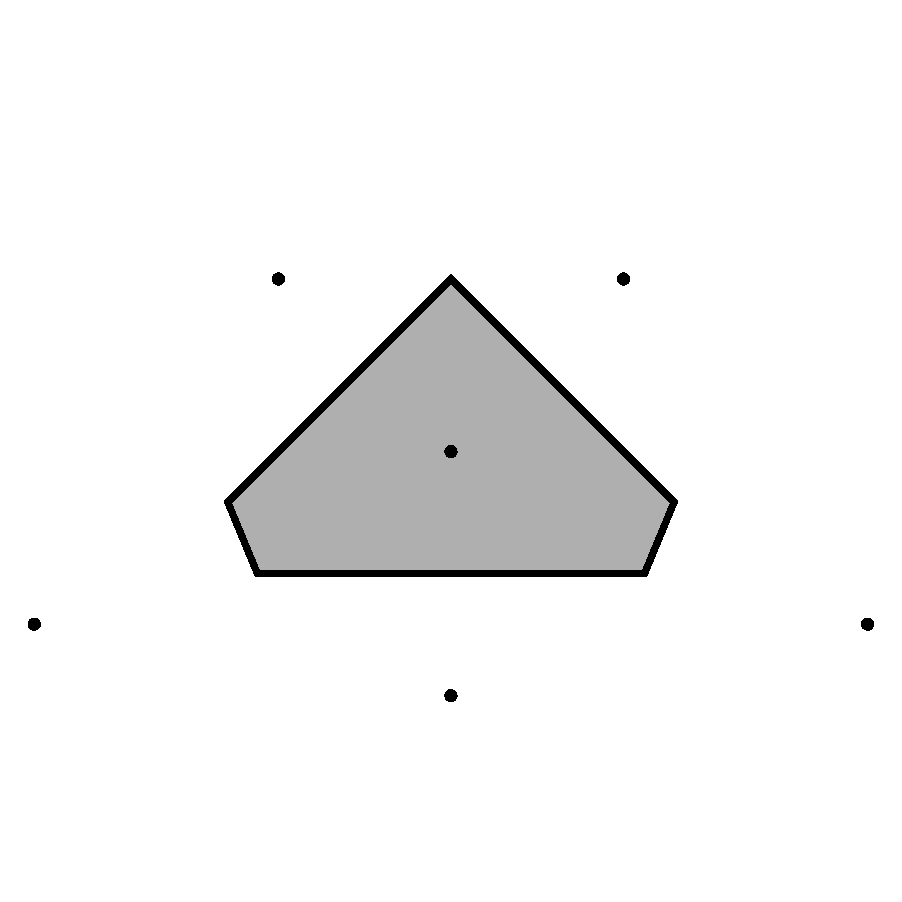
\includegraphics[width=0.2\textwidth]{img/2D/intersectionTile03}
\caption{The Voronoi tile for which we establish its period. }
\label{fig_example2D_tile}
\end{figure}

Octagon's area increases quadratically with increased length of its edge, therefore we will assume the following formula for area of the intersection $(\omega\Omega)|_V$: 
$$A = a(\omega+d)^2 \quad\text{for}\quad a,d,\omega\in\RR$$
If we know three pairs of $\omega$ and area of the corresponding intersection, we can calculate $a$ and $d$:
$$(x_1,A_1) \qquad (x_2,A_2) \qquad (x_3,A_3)$$
$$a = \frac{\frac{A_1-A_2}{x_1-x_2}-\frac{A_1-A_3}{x_1-x_3}}{x_2-x_3} \qquad d=\frac{A_1-A_2}{2a(x_1-x_2)}-\frac{x_1+x_2}{2}$$

Now to get $\omega_1$ we calculate the area $A((\omega\Omega)|_V)$ for three different values of $\omega$ and use the formulas above: 
\begin{align*}
x_1&=\frac{556-215\beta_8}{37} & A_1&=\frac{163521\beta_8-394721}{5476} \\
x_2&=\frac{546-211\beta_8}{37} & A_2&=\frac{159633\beta_8-385353}{5476} \\
x_3&=\frac{536-207\beta_8}{37} & A_3&=\frac{155793\beta_8-376097}{5476} \\
\end{align*}
$$a = \frac{1+3\beta_8}{2}$$
$$d = \frac{15-7\beta_8}{2}$$
We are looking for the area $A((\omega\Omega)|_V)$ to be zero:
$$\omega_1+d=0\quad\Rightarrow\quad \omega_1 = \frac{7\beta_8-15}{2}\doteq 0.94975$$

Even though this method seems to be theoretically sound, we could not get reliable results for $\omega_2$ this way. We presume that our precise arithmetic (Chapter \ref{cha_computation}) suffered from buffer overflow and thus we were not able to acquire $\omega_2$. That however is not a deal breaker for our overall analysis. 

\subsubsection{Circular window}
We could not use the approach we have just described for a circular window. Our program can do precise calculations only in $\field$ (Chapter \ref{cha_computation}) and we have not found a way to calculate an area of disc intersection in $\field$. There is however a direct way to calculate at least $\omega_1$. Essentially we are looking for a disc radius for which the intersection $\Omega|_V$ is a single point. After some consideration we arrive to the realization that $\Omega|_V$ is a single point if the radius is half of the distance between the centers of two furthest discs. Thus we can directly calculate $\omega_1$. 
\end{document}
